%%%%%%%%%%%%%%%%%%%% author.tex %%%%%%%%%%%%%%%%%%%%%%%%%%%%%%%%%%%
%
% sample root file for your "contribution" to a contributed volume
%
% Use this file as a template for your own input.
%
%%%%%%%%%%%%%%%% Springer %%%%%%%%%%%%%%%%%%%%%%%%%%%%%%%%%%


% RECOMMENDED %%%%%%%%%%%%%%%%%%%%%%%%%%%%%%%%%%%%%%%%%%%%%%%%%%%
\documentclass[graybox]{svmult}

% choose options for [] as required from the list
% in the Reference Guide

\usepackage{mathptmx}       % selects Times Roman as basic font
\usepackage{helvet}         % selects Helvetica as sans-serif font
\usepackage{courier}        % selects Courier as typewriter font
\usepackage{type1cm}        % activate if the above 3 fonts are
                            % not available on your system
%
\usepackage{makeidx}         % allows index generation
\usepackage{graphicx}        % standard LaTeX graphics tool
                             % when including figure files
\usepackage{multicol}        % used for the two-column index
\usepackage[bottom]{footmisc}% places footnotes at page bottom
%\usepackage{subcaption} %% ADDED
%%% Personal packages
%\usepackage[utf8]{inputenc}
\usepackage{longtable}
\usepackage{color}
\usepackage{multirow}
% see the list of further useful packages
% in the Reference Guide

\makeindex             % used for the subject index
                       % please use the style svind.ist with
                       % your makeindex program

%%%%%%%%%%%%%%%%%%%%%%%%%%%%%%%%%%%%%%%%%%%%%%%%%%%%%%%%%%%%%%%%%%%%%%%%%%%%%%%%%%%%%%%%%

\begin{document}
\tableofcontents

\title*{non-protein-coding RNAs as regulators of development in tunicates}


% Use \titlerunning{Short Title} for an abbreviated version of
% your contribution title if the original one is too long
\author{Cristian A. Velandia-Huerto, Federico D. 
Brown, Adriaan A. Gittenberger, Peter F. Stadler and Clara I. 
Berm\'{u}dez-Santana}
% Use \authorrunning{Short Title} for an abbreviated version of
% your contribution title if the original one is too long
\institute{Cristian A. Velandia-Huerto, \at {Bioinformatics Group, Department of 
Computer Science, and Interdisciplinary Center for Bioinformatics, 
Universit{\"a}t Leipzig},H{\"a}rtelstra{\ss}e 16--18, D-04107, Leipzig, Germany 
\email{cristian@bioinf.uni-leipzig.de}
\and Federico D. Brown \at Departamento de Zoologia, Instituto Bioci{\^e}ncias, 
    Universidade de S{\~a}o Paulo, Rua do Mat{\~a}o,  Tr. 14 no. 101,S{\~a}o 
Paulo, SP, Brazil \email{fdbrown@usp.br}
\and Adriaan A. Gittenberger \at Institute of Biology, Leiden University,P.O. 
Box 9505, 2300 RA, Leiden, Netherlands, \email{gittenberger@gimaris.com}
\and Peter F. Stadler \at {Bioinformatics Group, Department of Computer Science, 
and Interdisciplinary Center for Bioinformatics, Universit{\"a}t 
Leipzig},H{\"a}rtelstra{\ss}e 16--18, D-04107, Leipzig, Germany 
\email{studla@bioinf.uni-leipzig.de}
\and Clara I. Berm\'{u}dez-Santana \at Biology Department, Universidad 
Nacional de Colombia, Carrera 45 \# 26-85, Edif. Uriel Guti{\'e}rrez, 
\email{cibermudezs@unal.edu.co}
}

%
% Use the package "url.sty" to avoid
% problems with special characters
% used in your e-mail or web address
%
\maketitle

\abstract{Each chapter should be preceded by an abstract (10--15 lines long) 
that summarizes the content. The abstract will appear \textit{online} at 
\url{www.SpringerLink.com} and be available with unrestricted access. This 
allows unregistered users to read the abstract as a teaser for the complete 
chapter. As a general rule the abstracts will not appear in the printed version 
of your book unless it is the style of your particular book or that of the 
series to which your book belongs.
Please use the 'starred' version of the new Springer \texttt{abstract} command 
for typesetting the text of the online abstracts (cf. source file of this 
chapter template \texttt{abstract}) and include them with the source files of 
your manuscript. Use the plain 
\texttt{abstract} command if the abstract is also to appear in the printed 
version of the book.}


\section{Introduction}
\label{sec:1}

Tunicates are organisms characterized by a fast rate of genomic and 
developmental evolution. Some fast evolving evolutionary changes include loss of 
synteny, fast changes in \textit{cis}-regulatory sequences, and loss of several 
key regulatory developmental genes \cite{Satou2008, Denoeud1381}, such as 
several central or posterior Hox genes involved in AP patterning 
of metazoans \cite{Ikuta:2005} and Gbx involved in the establishment of 
the midbrain-hindbrain boundary in vertebrates \cite{Yagi2003}. Genome 
studies of miRNA prevalence in several species of tunicates (i.e.Oikopleura, 
Ciona and Didemnum) have revealed many losses of conserved miRNA families as 
well as many gains of unique miRNAs among recently divergent lineages in the 
tunicates when compared to other groups of chordates \cite{Fu2008, 
Velandia-Huerto2016}. Thus, relaxed constraints in the evolution of 
genomes and developmental trajectories in the tunicates may have been 
responsible for the plethora of reproductive strategies, morphologies, and life 
histories observed in the group \cite{Holland2015}.

noncoding RNAs roles in tunicates development date earliest in the 90`s from 
the works of Swalla \& Jeffry in which RNAs localized in the yellow crescent or 
myoplasm, a cytoskeletal domain in oocytes of the ascidian \textit{Styela clava} 
were discovered \cite{Swalla1995}. This  yellow crescent or YC RNA identified to 
be present throughout embryonic development was the first example involved in 
envisioning the future of a growing family of ncRNAs that would play important 
roles in growth and development in tunicates\cite{Swalla1995}.

This asymmetrically distributed ascidian RNAs were part of the set of many 
other RNAs known as maternally synthesized cytoplasmically localized RNAs, 
discovered first in oocytes of Xenopus \cite{Bashirullah1998}

\section{miRNA families origin and evolutionary perspective}
\label{sec:2}

\subsection{Origins and Evolution of MicroRNAs}

MicroRNAs (miRNAs) have been described in almost all animals and plants as
well as diverse unicellular eukaryotes. They are important
post-transcriptional regulators of gene expression affecting a sizable
fraction of all mRNAs \cite{Ameres:13}. Mechanistically, miRNAs depends on
the presence of the evolutionarily even older RNA interference pathways
\cite{Cerutti:06, Shabalina:08} that leads to the suppression of
double-stranded RNA molecules in a cell's cytoplasm. 

Throughout animals, canonical miRNAs are the processed through a
well-characterized pathway. The primary precursor transcript (pri-miRNA) is
transcribed by pol-II. While in most cases the pri-miRNA is a long
noncoding RNA, some miRNAs are processed from protein-coding transcripts,
where they are mostly derived from introns \cite{Lin:06}. In the next step,
hairpin-shaped precursors, the pre-miRNAs, are extracted while the RNA is
still residing in the nucleus. These are exported into the cytoplasm
\cite{Lund:04} and then processed further into miRNA/miRNA* duplexes.  In
the final step the single-stranded mature miR or its complement, the miR*,
is incorporated in RISC complex. Sequence complementarity of miR and mRNA
ensures the targeting specificity \cite{Bartel:13}. As as a consequence,
miRNAs share a set of structural characteristics, most importantly the
extremely stable secondary structure of the precursor hairpin and the 2-bp
overhang of miR and miR* generated by Dicer processing. These features make
it possible to reliably identify miRNAs from short RNA-seq data, see e.g.
\cite{Langenberger:10a, Friedlaender:12, Langenberger:13a}.

Most animal microRNAs are among the most highly conserved genetic elements.
The most stringent selection pressure acts on the mature miR sequence. This
is a consequence of the fact that a single miR typically targets a large
number of mRNAs. Mutations in the mature sequence thus simultaneous affect
many interactions, and thus are almost always selected against. In
conjunction with the stringent requirements on the secondary structure, the
entire precursor is under strong stabilizing selection \cite{Price:11},
explaining the observed high levels of sequence conservation. As a
consequence, even evolutionarily distant homologs of miRNAs can be readily
detected despite the short sequence length. Most efficiently,
\texttt{infernal} \cite{Nawrocki:13} is used for this purpose, since it
makes use of both sequence and structure comparison.  The evolution of
miRNAs can thus be traced back in time with high accuracy
\cite{Hertel:06a}. 

Like other gene families, miRNAs form paralogs \cite{Tanzer:04a, Hertel:12a}
and hence often appear as families as homologous genes. This forms the
basis of the \texttt{miRBase} nomenclature \cite{Ambrose:03a}. A series of
investigations into the phylogenetic distribution of miRNA families showed
that miRNAs are infrequently lost at family level and thus serve as
excellent phylogenetic markers
\cite{Sempere:06, Heimberg:08, Heimberg:10, Wheeler:09}, although the massive
restructuring of the miRNA complement of tunicates is an important
exception to this rule \cite{Fu:08}.

The innovation of new miRNA families is an on-going process. Experimental
surveys of the miRNA repertoir thus have reported a large number of very
young and even species-specific miRNAs \cite{Bentwich:05, Berezikov:06}. The
process was studied quantitatively in fruit flies, where innovation rate of
as many as $12$ new miRNA genes per million years has been estimated
\cite{Lu:08}. This is consistent with the fact that stable hairpins are
abundant structural elements in random RNAs, which makes is not only
possible but actually quite likely that miRNA precursors appear by chance
in transcribed genomic regions \cite{Tanzer:04a, CampoPaysaa:11, Marco:13}.
Of course, only a tiny fraction of these fortuitously processed hairpins
have a function and hance are subject to selection, and an even smaller
subset is conserved over long evolutionary time scales. Detailed studies
showed that evolutionarily young miRNA have comparably low expression
levels. Initially, they go through a phase of relatively fast sequence
evolution \cite{Liang:09, Meunier:12}, which slows down as the selective
pressures from a gradual increase in the number of target site increases. A
large, diverse set of targets then protects against miRNA loss
\cite{Lee:07a}. The rate of gain of miRNA families that retained
essentially permanently amounts to only $1$ per several million years. This
number is consistent with divergence of the miRNA complements between
animal phyla.

Many authors have observed that overall the miRNA repertoire has been
expansing throughout animal evolution in a manner that at least roughly
correlates with morphological complexity
\cite{Hertel:06a, Sempere:06, Niwa:07, Prochnik:07, Lee:07a, Heimberg:08, Peterson:09, Berezikov:11}. 
Several bursts of miRNA innovation have been observed
\cite{Hertel:06a, Heimberg:08, Tanzer:10a, Hertel:15a}, most notably at the
root of the placental mammals, the ancestor of ``free-living'' nematodes,
or the radiation of the drosophilids. Massive morphological simplification,
on the other hand, is sometimes associated with a drastic loss of miRNA
families. This has been observed most prominently for tunicates
\cite{Fu:08, Dai:09}.

%\subsection*{MicroRNAs in Tunicates} 

%\TODO{I think we do not really most of the papers below, since much of the
%  relevant material is already subsumed in the summary above.} 
%It was included on 'Validation and detection of miRNA families in Cionas in this decade' and 'The new era to get deep insights into the repertory of miRNA in other urochordates'.

\subsection{miRNA identification and validation}

The first microRNA (miRNA) in tunicates was discovered in the year 2000 from 
the work of \textit{Pasquinelli et al., 2000} when they were studying 
the temporal regulation of let-7 during development by using samples of small 
RNAs of a wide range of animal species, in which the ascidian \textit{Ciona 
intestinalis} was included as well as other vertebrates, hemichordates, mollusc, 
annelids, arthropod and other bilateral and nonbilateria animals 
\cite{Pasquinelli2000}. Later on the year 2003 the same team suggested that 
let-7 RNA may control the late temporal transitions during development across 
animal phylogeny \cite{Pasquinelli2003} albeit it was not identified on basal 
metazoans such as cnidarians and poriferans. 

Then after the era of genome sequencing became available, it was launched in 
2005 the computational screening of whole-genomes of non-model organism as 
tunicates. Beginning with the Cionas \textit{C. intestinalis} and \textit{C. 
savigni} a profile-based strategy was implemented in the ERPIN program 
\cite{Legendre2005}. On that work were detected a set of new miRNAs candidates 
considered as \textit{C. intestinalis} specific such as the members of the 
family miR-9 and miR-79 and as it was expected, other miRNA families were found 
homologous between both Cionas like the families miR-124;92;98;325;310-313 and 
let-7. Coincidentally, by the same year a whole-genomic comparative approach in 
the urochordate lineage was performed on the species \textit{C. intestinalis, C. 
savignyi} and \textit{O. dioica}. Using a computational screening of structured 
ncRNAs based upon homology between predicted precursor hairpin structures  $41$ 
miRNA candidates were detected including let-7 and other six known candidates in 
\textit{C. intestinalis} \cite{Missal2005}. After all, the same group in 2007 
implemented a structure-based clustering approach in \textit{C. intestinalis} 
predicted $58$ miRNAs, of which only let-7, miR-7, miR-124, and miR-126 
coincided with the previously annotated miRNAs \cite{Will2007}. 

Thus far, the primary focus to identify miRNAs into urochordate linage has been 
mainly toward the use of computational approaches but soon came up the use of 
new hybrid strategies combining computational and experimental studies to 
validate candidate families previously detected. For instance the first bona 
fide record for \textit{C. intestinalis} was registered in mirBase only in its 
Release 11. Those first miRNAs records were derived from the work published in 
2007 by Norden-Krichmar et al., \cite{Norden-Krichmar2007}. The authors searched 
for conservation with the seed region of the known mature miRNA sequences from 
miRBase release 2006 on the whole-genomic sequences of \textit{C. intestinalis} 
and \textit{C. savignyi}. Those miRNAs were aligned locally using the 
FASTA/ssearch34 program. Only matches of 90\% identity or better were retained. 
In further steps these authors studied RNA sequences that folds like hairpin 
structures with the mature miRNA sequence in the stem region including other 
typical features exhibit in miRNA hairpins. By manual curation of the genomic 
sequences predicted by the software mfold which folded like hairpin structures, 
a set of $18$ miRNA molecules were detected which appeared conserved in both 
Cionas. After all, using  Northern blot analyses in the adult tissue of 
\textit{C. intestinalis} the authors confirmed expression of  let-7, miR-7, and 
miR-126, as well as $11$ other conserved miRNA families.

Until 2008, most of the miRNAs annotations were concentrated in Cionas, but new 
annotation approaches for other species in tunicates were appearing slowly to 
increase then the repertory of new miRNAs families in urochordates. In this 
order of ideas, the first repertory of miRNAs based on non-Cionas species was 
published by Fu et al., in  2008 for the larvacean \textit{O. dioica} 
\cite{Fu2008}. At that time the authors were studying the temporal-spatial 
expression patterns of conserved miRNAs in different developmental stages of 
oocytes, 1-cell zygote, 2-8 cell embryons, blastulas, gastrulas, tadpoles (in 
different stages) and animals from 1 to 6 days from \textit{O. dioica}. In this 
research, small RNAs were isolated, amplified by RT-PCR and rapid amplification 
of cDNA ends (RACE) of the developmental stages, cloned and sequenced. Blast 
searches using the sequences of cloned small RNA libraries were used to annotate 
small RNAs as miRNA candidates. In further steps the recovered  genomic flanking 
sequences each side of those mapped candidates were used as input to predicted 
secondary structures by mfold v3.1. This step was used to detect candidates that 
folds like miRNA hairpins and aimed to decrease the set of false positive 
potential miRNAs in \textit{O. dioica}. Finally, for this set of potential 
candidates a developmental miRNA array dot blot analyses were performed to 
detect miRNA expression. With this approach from $3066$ sequenced small RNA 
clones only for $55$ miRNAs was detected expression. As a conclusion the authors 
suggested that those candidates were expressed throughout the short life cycle 
of \textit{O. dioica} showing that some of them were stocked as maternal 
determinants prior to rapid embryonic development.  Besides the authors 
identified a set of sex-specific miRNAs that appeared as male/female gonad 
differentiation which became apparent and was maintained throughout 
spermatogenesis \cite{Fu2008}. Unexpectedly, the majority of the miRNAs loci in 
\textit{O. dioica} were located in antisense orientations into the hosted genes 
in opposite fashion observed in the majority of the known mammalian miRNAs at 
that time. 

Between the years 2009 and 2015 the majority of the studies of miRNAs in 
tunicates were focused into the validation of expression of computational 
predicted miRNAs in Cionas specially focused in \textit{C. intestinalis} as 
model organism of tunicates or into the test of new computational approaches as 
miRTRAP, miRDeep2 and miRRim2 which used next-generation sequencing libraries of 
small RNAs derived from \textit{C. intestinalis} to validate their algorithms. 
Then by the year 2016 the first comparative homology based search strategy let 
us to identify the repertory on miRNAs and other ncRNAs in the carpet sea squirt 
\textit{Didemnum vexillum} with a preliminary comparative analysis of gain and 
losses of miRNA families on chordates which included the \textit{Cionas}, 
\textit{O. dioca} and the colonial tunicate \textit{Botryllus schlosseri} 
\cite{Velandia-Huerto2016}. By the same year, from the preliminary genome 
sequence assembled for the Southern Ocean salp, \textit{Salpa thompsoni} 
(Urochordata, Thaliacea) a set of miRNAs families were detected \cite{Jue2016} 
and in 2017 the prediction of miRNAs families were reported to the species 
\textit{Halocynthia roretzi}. On the following two sections we will focus on 
those stages of the fascinated increased screening of the miRNA repertory in 
tunicates.

\subsubsection{Validation and detection of miRNA families in Cionas in this decade}

At the end of the last decade the application of next generation sequencing 
technologies to sequence small RNA libraries changed the common way used to 
detect expression of miRNAs in many organisms including the tunicates. This 
technology became in one of the most common approaches that supported methods 
like RT-PCR, microarrays or dot blotting which were previously used to validate 
miRNA expression in tunicates. In 2009 after preparing small RNA libraries from 
various developmental stages including unfertilized eggs, early embryos, late 
embryos and adults from  \textit{C. intestinalis} was performed high-throughput 
sequencing of cDNA with an Illumina 1G Genome Analyzer experiments. These 
sequencing led to document $80$ miRNAs families for  \textit{C. intestinalis}. 
Unexpectedly, were detected a distinct species of small RNAs processed outside 
of the miRNA precursors which were termed as moRs or miRNA-offset RNAs 
\cite{Shi2009}. Later on, after extracting non-coding conserved regions of whole 
genome alignments between  \textit{C. intestinalis} and \textit{C. savigny} a 
set of $12$ million sequences were computationally folded using RNAfold and 
mfold. Then after combining the following criteria: structure/sequence 
conservation, homology to known miRNAs, and phylogenetic footprinting the 
authors detected a set of $458$ candidate sequences \cite{Keshavan2010}. Then 
in order to validate those candidate, RT-PCR and PAGE were conducted to design 
a custom microarray. After screened them for miRNA expression were identifying 
that $244$ of the $458$ miRNA predictions were represented either in their 
microarray data or in the Illumina database constructed previously for small RNA 
derived from \textit{C. intestinalis} by \cite{Shi2009}. Although they failed to 
predict $39$ previously characterized miRNAs, it was suggested in this work that 
\textit{C. intestinalis} genome may encode about $300$ miRNA genes. Then to 
increase the miRNAs collection in \textit{C. intestinalis} a novel computational 
strategy for the systematic, whole-genome identification of microRNA from high 
throughput sequencing information was developed in 2010 by \cite{Hendrix2010}. 
That method, known as miRTRAP, incorporated not only the mechanisms of microRNA 
biogenesis but also includes additional criteria regarding the prevalence and 
quality of small RNAs arising from the antisense strand and the neighboring 
loci. With that approach, nearly $400$ putative microRNAs loci were detected. In 
short words these strategy relies on the way how the the biochemical machinery 
processes pre-miRNA hairpins produces short RNA products. This approach is 
highly depended on the deep of the small RNAs mapped to a given locus and is 
highlighted by the authors that the approach requires an accurate assignment of 
small RNA sequences on their relative positions along the hairpin, that is, 
miR/miR*, moR/moR* and loop \cite{Hendrix2010}. Again a new approach took 
advantage of importance to detect miRNAs from the high-throughput sequencing of 
small RNAs available from \cite{Shi2009}. These approach known as  miRDeep2 
improved the algorithm of its first version miRDeep \cite{Friedlaender:12} and 
let to identify with an accuracy of $98.6$\% and $99.9$\% canonical and 
non-canonical miRNAs in different species. These approach reported $313$ known 
and $127$ novel ones miRNAs in \textit{C. intestinalis}. In the same year the 
program miRRim2 \cite{Terai2012} was applied to the \textit{C. intestinalis} 
genome, in which some candidates identified from the work of \cite{Hendrix2010} 
and the several promising candidates were detected. In 2013, \cite{Kusakabe2013} 
was investigated the expression patterns of the cluster miR-1 and miR-133 in 
\textit{C. intestinalis} and in \textit{C. savignyi}. RT-PCR amplification of 
miR-1/133 precursors were performed and PCR products were subcloned and 
sequenced. Whole-mount in situ hybridization to detect cin-miR-1/miR-133 primary 
transcript was performed and LNA Northern blotting was conducted on different 
developmental stages. 

\subsubsection{The new era to get deep insights into the repertory of miRNA in other urochordates}

Since 2016 new approximations has increased our knowledge about new families in 
other tunicates thanks to the sequence of new urochordate genomes of the species 
\textit{D. vexillum}, \textit{S. thompsoni} and \textit{H. roretzi} %do not know 
write here B. schlosseri because no-ncRNAs were reported, only on mtDNA and 
methodology to validate genes by RNA-seq from different tissues and it was 
reported on 2013...

(Please summary of our Dvexillum paper \cite{Velandia-Huerto2016} including the 
first reported preliminary annotation for colonial tunicate \textit{B. 
schlosseri} beside the one for Dvexillum.)
%%%%ADDED CRISTIAN
For the draft genome sequence from \textit{D. vexillum} an 
homology-based computational approach was applied \cite{Velandia-Huerto2016}. 
Blast and HMMer searches were performed with annotated small ncRNAs sequences 
from metazoans and hidden markov models from 
RFAM\footnote{\url{http://rfam.xfam.org/}} to obtain the sort of candidates at 
sequence level. Structural alignments of those sequences were performed by 
infernal (CITE), using metazoan-specific covariance models to annotate the small 
ncRNAs collection, which $57$ families and $100$ loci of miRNAs were found. 
%%%%%%%%%%%%

For the preliminary assembled of the genome sequence for the 
Southern Ocean salp \textit{S. thompsoni} \cite{Jue2016} were small RNA 
libraries constructed to be sequenced on an Illumina Hiseq 2000. After filtering 
data sets to 18-24 nt for miRNA and 28-32 nt for piRNA, the reads were aligned 
to \textit{S. thompsoni} genome and miRNA gene folding predictions were 
performed using RNAfold. In this initial survey of small RNAs, were revealed the 
presence of known, conserved miRNAs, as well as novel miRNA genes and mature 
miRNA signatures for varying developmental stages. Then in 2017, the prediction 
of $319$ miRNAs candidates in \textit{H. roretzi} were obtained through three 
complementary methods. The experimental validation suggested that more than half 
of these candidate miRNAs are expressed during embryogenesis. The expression of 
some of the predicted miRNAs were validated by RT-PCR using embryonic RNA. In 
this approach \textit{C. robusta} small RNA-Seq reads derived from \textit{C. 
robusta} \cite{Shi2009} (previously known as  \textit{C. intestinalis} today 
reclassified) was used to identify conserved miRNAs in \textit{H. roretzi} 
\cite{Wang2017}.


\subsection{miRNA in clusters}

One of the most interesting aspects about the patterns of genomic locations of 
miRNAs is to known whether those loci are randomly distributed throughout the 
genome as single copies or if they are arranged on consecutive locations or in 
tandem copies clustered to be expressed from polycistronic primary precursors or 
to be transcribed independently. Interestingly in \textit{O. dioca} miRNAs are 
located in the antisense orientations of protein-coding gene and immediately 
downstream of its corresponding 3`UTR region or even more in the sense strand of 
introns \cite{Fu2008}. Nevertheless, after those conspicuous distributions some 
clusters have been also identified in \textit{O. dioca}. For instance four 
miRNAs, miR-1490a, miR-1493, miR-1497d, and miR-1504, are reported by 
\cite{Fu2008} to be presented as two copies, and miR-1497d-1 and miR-1497d-2 are 
included in the large miR-1497 cluster. See the current structure of this 
cluster in Table \ref{tab:detailBigClusters} although only one copy for the  
miR-1497 has been reported for \textit{C. instestinalis} located in an 
intergenic region \cite{Fu2008}, \cite{Hendrix2010} and one in \textit{C. 
savigny} overlapped in an intron \cite{Fu2008}. By testing real time PCR 
co-expression of some miRNAs, their host and adjacent genes in \textit{O. dioca} 
by \cite{Fu2008} it was discovered for the case of the cluster  
miR-1487/miR-1488 a not clear positive or negative correlation with the 
expression of its anti-sense hosting gene. In males this cluster expression was 
not associated with the expression of its adjacent ABCA3 gene by the same 
authors.  

%%%
\begin{small}
\begin{center}
\begin{longtable}{p{2.0 cm}p{2 cm}p{2 cm}p{2 cm}p{1.2 cm}p{1.0 cm}p{2.6 cm}}
\caption{Details of biggest miRNA cluster for chordate species.}
\label{tab:detailBigClusters}
%\hline\noalign{\smallskip}
\tabularnewline
\hline\noalign{\smallskip}
\textbf{Specie} & \textbf{Chr} & \textbf{Start} & \textbf{End} & \textbf{Size (Mb)} & \textbf{No.} & \textbf{miRNAs detail} \\
\hline\noalign{\smallskip}
%\noalign{\smallskip}\svhline\noalign{\smallskip}
\textit{B. floridae} & Bf\_V2\_118 & $216744$ & $220351$ & $3607$ & $5$ & bfl-mir-4869, bfl-mir-4857, bfl-mir-4862, bfl-mir-4856b, bfl-mir-4856a \\
\textit{O. dioica} & scaffold\_3 & $2222857$ & $2223714$ & $857$ & $6$ & odi-mir-1497e, odi-mir-1497d-2, odi-mir-1497d-1, odi-mir-1497c, odi-mir-1497b, odi-mir-1497a \\
\textit{B. schlosseri} & chrUn & $40003$ & $41320$ & $1317$ & $2$ & mir-233, mir-10 \\
\textit{C. intestinalis} & $7$ & $4153284$ & $4156782$ & $3498$ & $23$ & cin-mir-4006d, cin-mir-4006c, cin-mir-4001b-2, cin-mir-4000i, cin-mir-4006g, cin-mir-4001e, cin-mir-4001d, cin-mir-4000g, cin-mir-4006f, cin-mir-4006b, cin-mir-4001b-1, cin-mir-4000c, cin-mir-4006e, cin-mir-4000b-2, cin-mir-4001a-1, cin-mir-4000b-1, cin-mir-4002, cin-mir-4000d, cin-mir-4001h, cin-mir-4000a-2, cin-mir-4006a-2, cin-mir-4006a-3, cin-mir-4006a-1 \\
\textit{C. savignyi} & reftig\_16 & $3924783$ & $3925336$ & $553$ & $3$ & csa-mir-216b, csa-mir-216a, csa-mir-217 \\
\textit{C. savignyi} & reftig\_1 & $1335375$ & $1336487$ & $1112$ & $3$ & csa-mir-92b, csa-mir-92c, csa-mir-92a \\
\textit{D. rerio} & $4$ & $28738556$ & $28754891$ & $16335$ & $60$ &  \small{dre-mir-430a-18, dre-mir-430c-18, dre-mir-430b-4, dre-mir-430a-15, dre-mir-430c-18, dre-mir-430b-5, dre-mir-430a-10, dre-mir-430c-18, dre-mir-430b-5, dre-mir-430a-15, dre-mir-430c-18, dre-mir-430b-3, dre-mir-430a-10, dre-mir-430c-18, dre-mir-430b-8, dre-mir-430a-15, dre-mir-430c-18, dre-mir-430b-5, dre-mir-430a-17, miR-430, dre-mir-430b-20, dre-mir-430a-10, dre-mir-430c-18, dre-mir-430b-5, dre-mir-430i-3, dre-mir-430c-18, dre-mir-430b-3, dre-mir-430a-10, dre-mir-430c-18, dre-mir-430b-8, dre-mir-430a-11, dre-mir-430c-18, dre-mir-430b-5, dre-mir-430i-3, dre-mir-430c-18, dre-mir-430b-19, dre-mir-430a-10, dre-mir-430c-18, dre-mir-430b-5, dre-mir-430a-17, miR-430, dre-mir-430b-20, dre-mir-430a-10, dre-mir-430c-18, dre-mir-430b-5, dre-mir-430i-3, dre-mir-430c-18, dre-mir-430b-19, dre-mir-430a-10, dre-mir-430c-18, dre-mir-430b-5, dre-mir-430a-15, dre-mir-430c-18, dre-mir-430b-3, dre-mir-430a-10, dre-mir-430c-18, dre-mir-430b-8, dre-mir-430a-15, dre-mir-430c-18, dre-mir-430b-5} \\
\textit{L. chalumnae} & JH126646.1 & $1529355$ & $1882777$ & $353422$ & $7$ & mir-233, mir-233, mir-233, mir-598, mir-672, MIR535, mir-233 \\
\hline\noalign{\smallskip}
\end{longtable}
\end{center}
\end{small}
%%

In \textit{C. intestinalis} some miRNAs are also located in introns and a small 
class of miRNAs are found to be deriving from mature mRNAs encoded within exons 
or UTR sequences \cite{Hendrix2010} in contrast to the location of the  loci in 
antisense orientations of protein-coding gene as seen in \textit{O. dioca} but 
this antisense orientation is reported for some miRNAs loci which express 
antisense miRs derived from miRNA loci as antisense products and antisense moR 
products as the miR-2246. Only $44$ loci appeared to be expressed as antisense 
products from the $300$ miRNA loci predicted in 2010 by \cite{Hendrix2010}. In 
Cionas have been also detected miRNAs organized in clusters, for example in  
\textit{C. intestinalis} a putative cluster was detected by \cite{Keshavan2010} 
using microarray analysis that shows a similar loci organization to the cluster 
let-7/miR-125/miR-100 observed in Drosophila. The miR-1473 was later classified 
as the orthologue of miR-100 in the analysis derived from the comparison of the 
evolution of this cluster conducted by \cite{Griffiths-Jones2011}. The authors 
suggested that mir-100, mir125 and let7 are clustered in most of the bilaterian 
genomes including as 1473 as orthologue of mir-100. 

\iffalse
\textcolor{red}{My main concerns here that the cluster 
let-7/miR-125/miR-100 observed in Drosophila and is included time ago for 
\cite{Griffiths-Jones2011}. In his plot you see a cluster on the right side 
and another on the left side, I am not sure why the mir-125 is not including 
if right now is validated in miRBAse shaping a cluster 
\ref{let7-mir125-mir1473}. Why the mir125 is not here? If it is reported time 
ago and is validated in miBase and by \cite{Keshavan2010}? And why mir233 is 
on it and not for Csa and Cin?. Please could you check this let7 cluster in 
the current plot?. Here I follow with Cristan description of this cluster. 
Please check about the mir125 and do any reconciliation if is posible with the 
plot of the paper of  \cite{Griffiths-Jones2011} in \ref{evolutionlet7}.}
\fi

%%CAVH response:
% For the case of Ciona intestinalis, the genome where the miRNAs had been 
%annotated on miRBAse is the JGI12, it is the genome from (Ensembl release 54) 
%OLD version. All the pipeline was executed on Ensembl release 81 (Bioinf 
%Colombia genome version).
% Specifically for the let-7/miR-125/miR-10 I review my data and the let-7 in 
%this genome where annotated as pseudogen because it did not report a greater 
%bitscore than the gathering score. But at now, it is included.

Current analysis of this cluster shows that the distribution of miRNAs families 
on this let-7 cluster are distributed in all the studied chordate species. In 
vertebrate species like (\textit{D. rerio} and \textit{L. chalumnae}) exists 
more than one let-7 cluster, extending the loci definition which is not 
restricted only for one element but for a cluster of many locus with different 
length distributions. It is important to see that let-7 is organized sometimes 
with another let-7 locus or with another miRNA's loci families. The distribution 
of this cluster reported on amphioxus is composed by 2 let-7 and 3 mir-10 (1 
bfl-mir-100, 1 bfl-mir-125a and 1 bfl-mir-125b), this 
cluster architecture almost conserved on vertebrates that apparently inverted 
the order and split the relation between let-7 and mir-10, creating two 
different cluster order groups: let-7 + mir-10 and let-7 + other families. 
In this way, tunicates reported the latter group, not including mir-10 on the 
cluster but including mir-233, mir-1473 or mir-125. 

A second miRNA cluster consisting of the miR-182 and miR-183 was also detected 
in \textit{C. intestinalis} in 2010 by \cite{Keshavan2010} which is in the 
current predictions is reported another member locus the miR-96 organized in the 
middle of those loci as is shown in the plot \ref{fig:mir-96}. 
Here the authots also found five additional paralogs of let-7 within a 1-kb 
stretch, but it is important to know that those elements had been identified on 
chromosome 4q on Ensembl release 54 version, at the current version only 
two of those elements have been identified by homology approaches (Figure 
\ref{fig:let-7}).

%Here the authors also found five additional paralogs of let-7 within a 1-kb 
%stretch previously know as Scaffold\_138 which is right now described on the 
%chromosome 4q. The current distribution for both Cionas is shown in 
%\ref{let7paralogs}. 

%\textcolor{red}{Unfortunately is not seen in the Cristian detection method?, 
%could we plotted or is not making sense? Since let7 is a very important 
%regulator of development (MAPPING, problem with mapping...)}
%%CAVH response:
%It does not generated results when I map the sequences against the current 
%genome version. Also in Ensembl is reported in the current genome:
%http://www.ensembl.org/Ciona_intestinalis/Location/View?r=4:2157322-2158920;db=
%core
%In this case, maybe is important to report this data as a complement...

The cluster miR-1/miR-133, expressed specifically in Cionas muscle tissues was 
also reported by \cite{Kusakabe2013}. The authors reported that one copy of this 
cluster is presented in both Cionas. As is shown in the plot 
\ref{fig:mir-1} a copy is also presented in \textit{L. chalumnae}. In 2012 a 
new cluster was proposed in \textit{C. intestinalis} by \cite{Terai2012} located 
on the cromosome 10q and composed by the mir-4054 locus and the mir-4091. In 
the current distribution of this cluster a new annotated family the mir-4008 
with three paralogous is located on the middle of those loci. This current 
distribution in shown of Table \ref{tab:otherClusters} whose loci were  
validated by \cite{Norden-Krichmar2007}, \cite{Fu2008}, \cite{Hendrix2010}, and 
\cite{Terai2012}. As was mentioned by \cite{Hendrix2010} is not very common to 
find related miRNAs organized in clusters composed by closely related families 
that differ in just a single nucleotide in the seed sequence as was found on the 
cluster composed by nine Ci-mir-2200, seven Ci-mir-2201 and nine Ci-mir2203 
which were previously reported under that putative names. They also found a 
second large cluster composed of $11$ miRNAs that gather into $4$ paralogous 
families three of Ci-mir-2200, three Ci-mir-2201, four Ci-mir-2204 and two 
Ci-2217. Current distribution of miRNAs families in \textit{C. intestinalis} and 
curated annotations indicate than in other regions of the chromosome 7q are also 
organized miRNAs in tandem copies of families. For instance the big cluster 
presumably re-named from \cite{Hendrix2010} today is known to be built by the 
families miR4000, miR-4001, miR4002, and miR4006 located on chromosome 7q 
(Table \ref{tab:otherClusters}). Another cluster is also located on the same 
chromosome composed by the families miR-4003, miR4005 and miR4077 in Table 
\ref{tab:otherClusters}. Some other cluster are also found on the cromosome 1a, 
10q and 3p. See this structure on Table \ref{tab:otherClusters}, most 
of them validated by \cite{Hendrix2010}. 

%\textcolor{red}{Please check the Table 
%\ref{tab:detailBigClusters} which are and which are not to update} 
%CAVH RESPONSE: ALREADY CHECKED AND UPDATED see table 2.

Some other clusters shared between both Cionas are the cluster 92, 124 and 200  
validated by \cite{Norden-Krichmar2007}, \cite{Fu2008}, \cite{Hendrix2010} which 
the structure is seen on Table \ref{tab:otherClusters}.    

%%%%

\begin{figure}[ht!]
\sidecaption[t]
%\centering
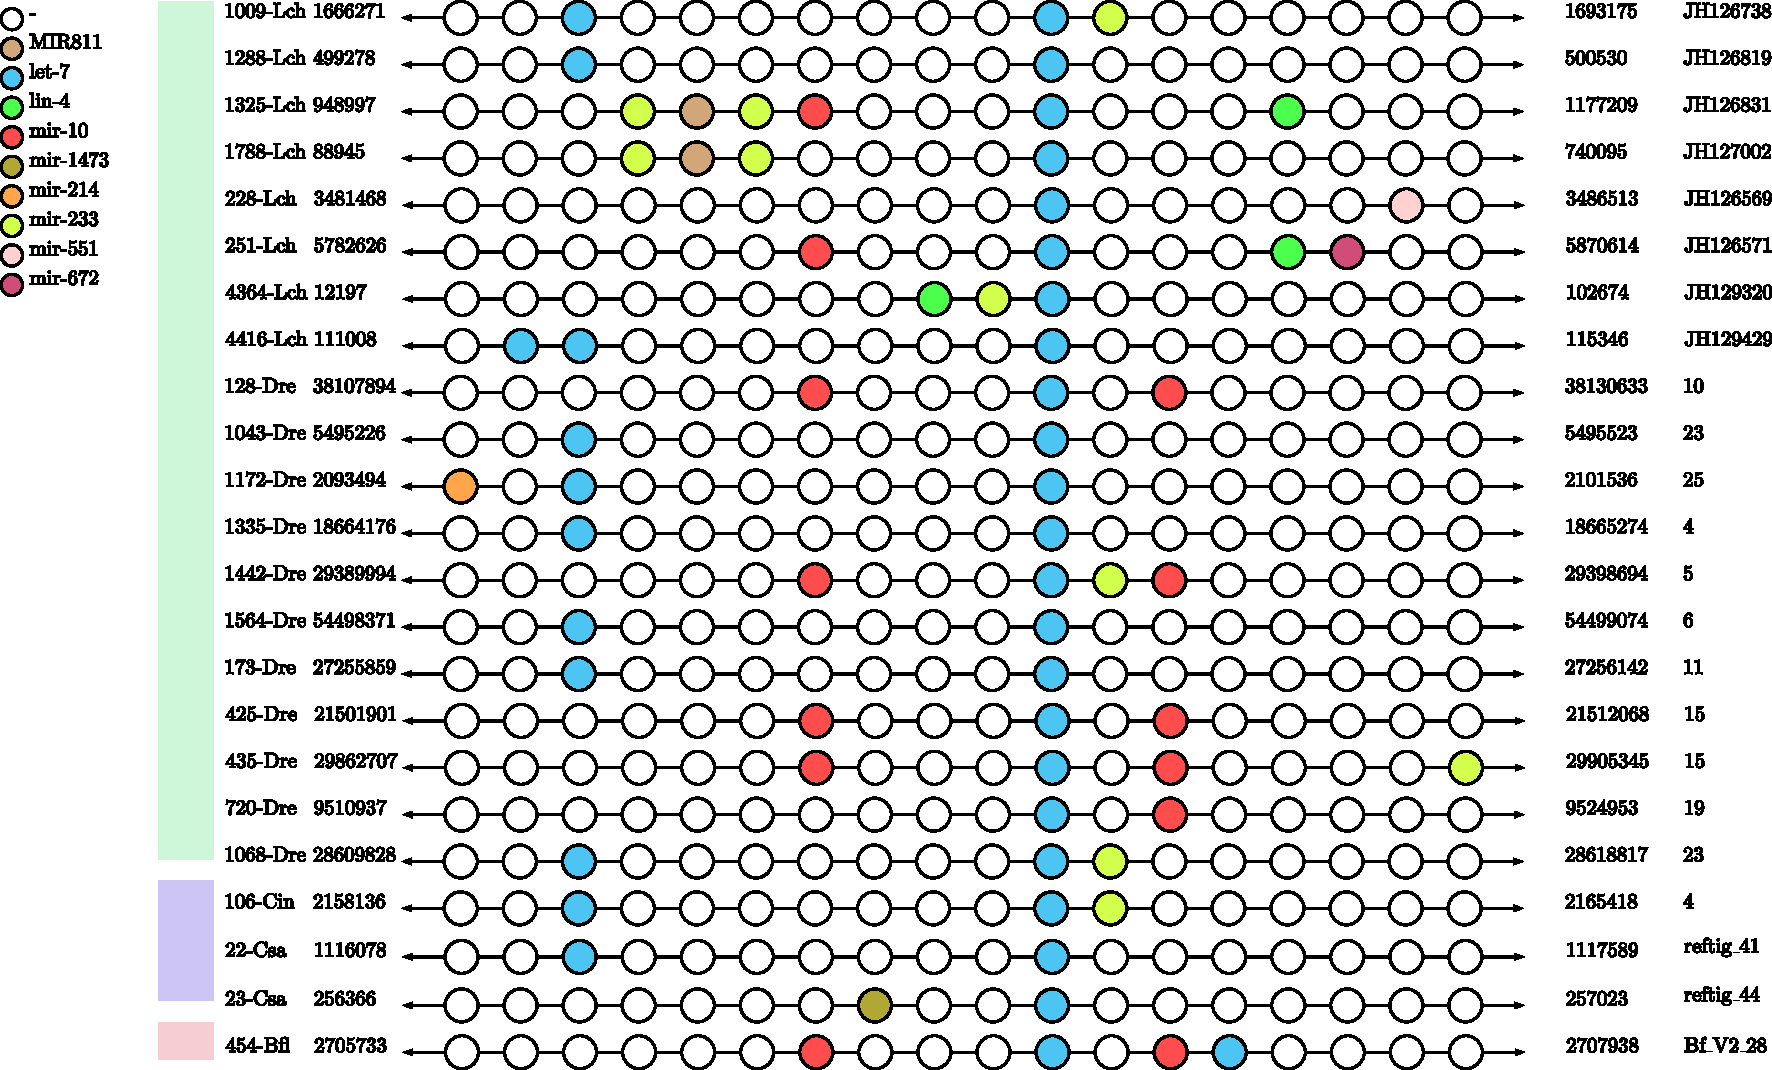
\includegraphics[width=\textwidth]{./Images/Cluster_images/let-7_101_128}
\caption{Multiple alignment of let-7 clusters. Specific names from annotations 
and homology predictions are described at the legend. Names from miRBase 
families are reported at the bottom of the aligned elements.} 
%the relationships between names and families had been found from this file:
%ftp://mirbase.org/pub/mirbase/CURRENT/miFam.dat.gz
\label{fig:let-7}
\end{figure}

\begin{figure}[ht!]
\sidecaption[t]
%\centering
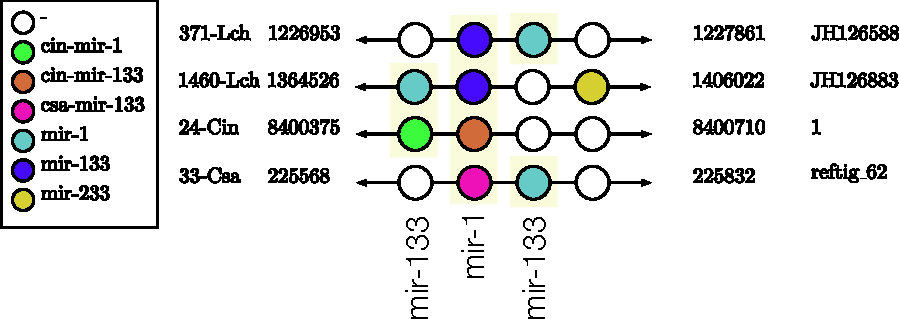
\includegraphics[width=\textwidth]{./Images/Cluster_images/mir-133_113_33}
\caption{mir-1/mir-133}
\label{fig:mir-1}
\end{figure}

\begin{figure}[ht!]
\sidecaption[t]
%\centering
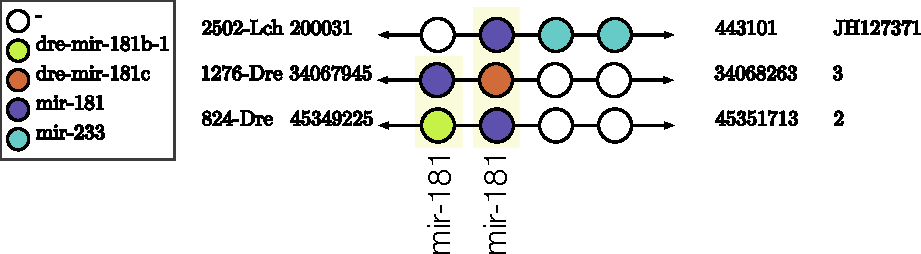
\includegraphics[width=\textwidth]{./Images/Cluster_images/mir-181_105_2502}
\caption{mir-181}
\label{fig:mir-1}
\end{figure}

\begin{figure}[ht!]
\sidecaption[t]
%\centering
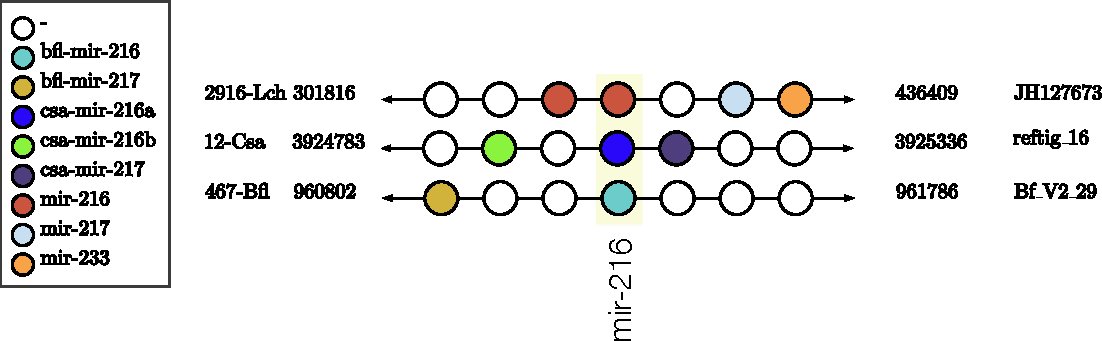
\includegraphics[width=\textwidth]{./Images/Cluster_images/mir-217_13D_467}
\caption{mir-216/mir-217}
\label{fig:mir-216}
\end{figure}

\begin{figure}[ht!]
\sidecaption[t]
%\centering
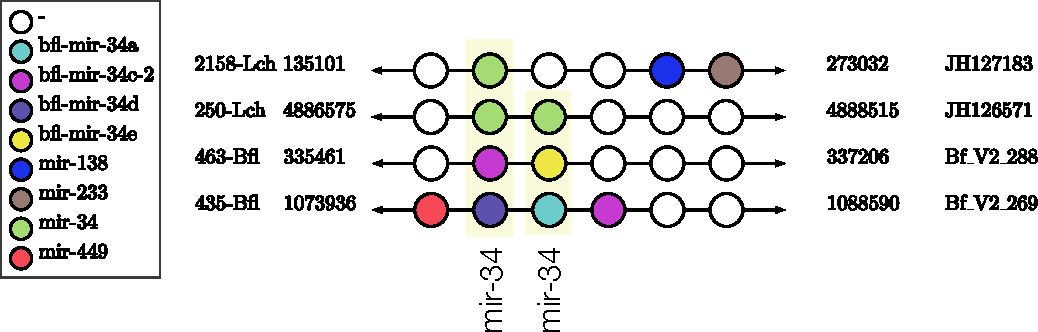
\includegraphics[width=\textwidth]{./Images/Cluster_images/mir-34_11A_435}
\caption{mir-34}
\label{fig:mir-34}
\end{figure}

\begin{figure}[ht!]
\sidecaption[t]
%\centering
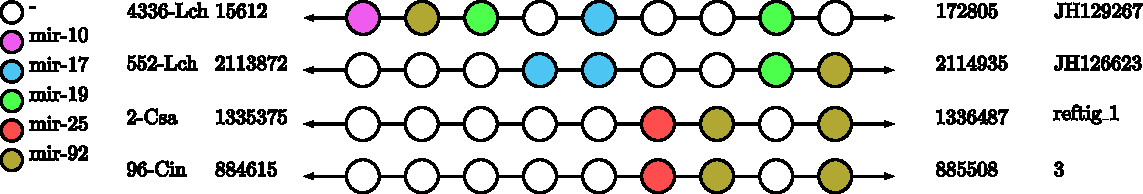
\includegraphics[width=\textwidth]{./Images/Cluster_images/mir-92_281_4336}
\caption{mir-92}
\label{fig:mir-92}
\end{figure}

\begin{figure}[ht!]
\sidecaption[t]
%\centering
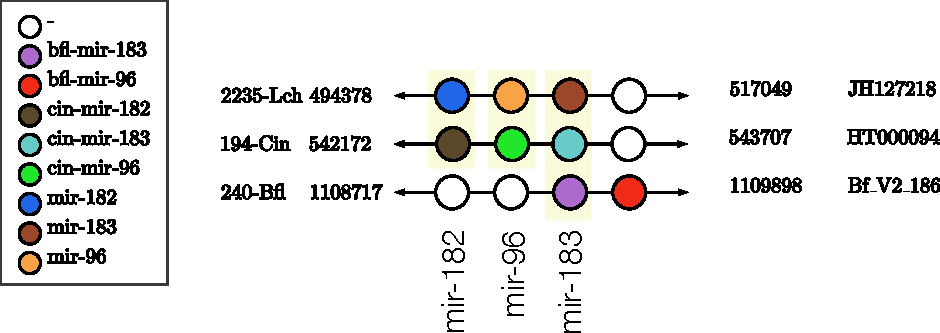
\includegraphics[width=\textwidth]{./Images/Cluster_images/mir-96_138_240}
\caption{mir-182/mir-96/mir-183}
\label{fig:mir-96}
\end{figure}

%\caption{Multiple alignments of miRNA's clusters. \textbf{Prot}: 
%Protostomata, \textbf{Brfl}: \textit{B. floridae}, 
%\textbf{Oidi}: \textit{O. dioica}, \textbf{Dvex}: \textit{D. vexillum}, 
%\textbf{Ciin}: \textit{C. intestinalis}, \textbf{Cisa}: \textit{C. savignyi}, 
%\textbf{Ciro}: \textit{C. robusta}, \textbf{Sath}: \textit{S. thompsoni}, 
%\textbf{Mata}: \textit{M. oculata}, \textbf{Mlta}: \textit{M. occulta}, 
%\textbf{Mlis}: \textit{M. occidentalis}, \textbf{Bosc}: \textit{B. schlosseri}, 
%\textbf{Haro}: \textit{H. roretzi}, \textbf{Pema}: \textit{P. marinus}, 
%\textbf{Dare}: \textit{D. rerio}, \textbf{Lach}: \textit{L. chalumnae}, 
%\textbf{Xetr}: \textit{X. tropicalis} and \textbf{Anca}: \textit{A. 
%carolinensis}.}
%\end{figure}

\begin{small}
\begin{center}
\begin{longtable}{lclllp{2.5cm}p{3cm}p{2.5cm}p{1cm}}
\tabularnewline
\caption{Reported clusters on literature. Bold text represent those miRNAs 
elements that are currently annotated and validated, but could not 
possible to detect by homology strategies.} %Here I reported my calculated 
%coordinates, miRBase ones are mostly to far from Ensembl ones.}
\label{tab:otherClusters}
%\hline\noalign{\smallskip}
\tabularnewline
\cline{1-9}
\textbf{Family} & \textbf{Specie} & \textbf{Chr} & \textbf{Start} & \textbf{End} 
& \textbf{miRNAs} & \textbf{Comments} & \textbf{Source DB} & 
\textbf{Ref.}\\
\tabularnewline
\cline{1-9}
\multirow{2}{*}{let-7} & Ciin & 4q & $2082260$ & $2083286$ & 
\textbf{cin-let-7a-1, cin-let-7f, cin-let-7b, cin-let-7c, cin-let-7a-2} & 
Reported on miRBAse and annotated on Ensembl & miRBase & \cite{Hendrix2010}, 
\cite{Fu2008} \\
 & Cisa & reftig\_41 & $1114139$ & $1117597$ & \textbf{csa-let-7c-1, 
csa-let-7b, csa-let-7a, csa-let-7c-2} & Reported on miRBase and does not 
detected by homology strategies. & miRBase & \cite{Fu2008} \\
\hline
mir-4091 & Ciin & 10q & $3226200$ & $3228884$ & \textbf{cin-mir-34}, 
cin-mir-4091, cin-mir-4008a, cin-mir-4008c, cin-mir-4008b, cin-mir-4054 & NA & 
miRBase and Homology & \cite{Norden-Krichmar2007}, \cite{Fu2008}, 
\cite{Hendrix2010}, and \cite{Terai2012}\\
\hline
7qother & Ciin & 7q & $4828431$ & $4835967$ & cin-mir-4077b, cin-mir-4003b, 
cin-mir-4005b, cin-mir-4077d, cin-mir-4003a-1, cin-mir-4003c, cin-mir-4077a, 
cin-mir-4003a-4, cin-mir-4003d & NA & miRBase and Homology & 
\cite{Hendrix2010} \\
\hline
3p & Ciin & 3q & $567478$ & $571031$ & cin-mir-4001f, cin-mir-4000e, 
cin-mir-4001c, cin-mir-1502d, cin-mir-4018a, cin-mir-4019, cin-mir-1502b, 
cin-mir-1502a, cin-mir-4007, cin-mir-4000f, cin-mir-4001i, cin-mir-4018b, 
cin-mir-1502c & Inclusion of cin-mir-4019 and cin-mir-4007  & miRBase and 
Homology & \cite{Hendrix2010} \\ 
\hline
1q & Ciin & HT000037.1 & $4884$ & $5250$ & \textbf{cin-mir-367}, 
\textbf{cin-mir-4009c}, \textbf{cin-mir-4009b}, cin-mir-367, cin-mir-4009c, 
cin-mir-4009a, cin-mir-4009b & Non-highlighted names could be found in the 
current genome at HT000037.1 scaffold & miRBase and Homology & 
\cite{Hendrix2010} \\
\hline
10q & Ciin & 10q & $3226200$ & $3228884$ & \textbf{cin-mir-34}, cin-mir-4091, 
cin-mir-4008a, cin-mir-4008c, cin-mir-4008b, cin-mir-4054 & NA & miRBase and 
Homology & \cite{Hendrix2010} \\
\hline
\multirow{3}{*}{mir-92} & Ciin & 3q & $884615$ & $885508$ &
cin-mir-92a, cin-mir-92d, cin-mir-92c & NA & miRBase and Homology & 
\cite{Hendrix2010} \\
 & Cisa & reftig\_1 & $1335375$	& $1336487$ & csa-mir-92b, 
csa-mir-92c, csa-mir-92a & NA & miRBase and Homology & \cite{Fu2008} \\
 & Oidi & scaffold\_1 & $3086369$ & $3086586$ & odi-mir-92b, odi-mir-92a & NA 
& Homology & \cite{Fu2008} \\
\hline
\multirow{2}{*}{mir-124} & Ciin & 7q & $4969691$ & $4969912$ & cin-mir-124-1, 
cin-mir-124-2 & NA & miRBase and Homology & \cite{Hendrix2010}, \cite{Fu2008} \\
& Cisa & reftig\_262 & $49392$ & $49620$ & csa-mir-124-1, 
csa-mir-124-2 & NA & miRBase and Homology & \cite{Fu2008} \\
\hline
\multirow{2}{*}{mir200} & Ciin & HT000325.1 & $8331$ & $8778$ & 
cin-mir-200, \textbf{cin-mir-3575}, cin-mir-141, \textbf{cin-mir-5611} & NA & 
miRBase and Homology &  \cite{Norden-Krichmar2007}, \cite{Fu2008}, 
\cite{Hendrix2010}, \cite{Friedlaender:12} \\
& Cisa & reftig\_613 & $31353$ & $31949$ & csa-mir-200, 
csa-mir-141 & NA & miRBase and Homology & \cite{Fu2008} \\
7qf & Ciin & 7q & $4153284$ & $4156782$ & cin-mir-4006d, cin-mir-4006c, 
cin-mir-4001b-2, cin-mir-4000i, cin-mir-4006g, cin-mir-4001e, cin-mir-4001d, 
cin-mir-4000g, cin-mir-4006f, cin-mir-4000h*, cin-mir-4006b, cin-mir-4001b-1, 
cin-mir-4006e, cin-mir-4001a-1, \textbf{cin-mir-4001a-2}, cin-mir-4002, 
cin-mir-4001h, 
cin-mir-4000a-2, cin-mir-4006a-2, cin-mir-4006a-3, cin-mir-4006a-1, 
\textbf{cin-mir-4006e}, \textbf{cin-mir-4001a-1}, \textbf{cin-mir-4006b}, 
cin-mir-4000c, \textbf{cin-mir-4006e}, cin-mir-4000b-2*, 
\textbf{cin-mir-4001a-1}, cin-mir-4000b-1*, \textbf{cin-mir-4001a-2}, 
\textbf{cin-mir-4002}, cin-mir-4000d*, \textbf{cin-mir-4001h}, 
\textbf{cin-mir-4006a-3}, \textbf{cin-mir-4006a-1}, \textbf{cin-mir-4000a-1} & 
Elements marked with * are identified by homology strategies at the same 
cluster, but in another order reported by miRBase. & 
miRBase and Homology & \cite{Hendrix2010} \\
\cline{1-9}
\end{longtable}
\end{center}
\end{small}

\iffalse
\subsubsection{Yanetal2014.pdf}

\cite{Yang2014}
\textit{mir181 is an ancient microRNA (miRNA) gene family that originated in urochordata. Although their functions were subjected to extensive studies in recent years, their evolutionary process remains largely unknown. Here we systematically investigated the homologous genes of the mir-181 family by a sequence similarity search. Representative sequences of the mir-181 gene family were used to reconstruct their evolutionary history. Our results indicated that this family could have derived from multiple duplications, which include two rounds of whole genome duplications and one round of segmental replication. Functional annotation of the target genes of the mir-181 family suggested that this family could participate in some important biological processes including transcriptional and translational regulation, signaling transduction etc. This analysis presented a complex evolutionary dynamics for the origination of a miRNA gene family.}

\subsubsection{Wangetal2017.pdf}
cite{Wang2017}
\textit{Background: miRNAs play essential roles in the modulation of cellular functions via degradation and/or translation
attenuation of target mRNAs. They have been surveyed in a single ascidian genus, Ciona. Recently, an annotated
draft genome sequence for a distantly related ascidian, Halocynthia roretzi, has become available, but miRNAs in
H. roretzi have not been previously studied.
Results: We report the prediction of 319 candidate H. roretzi miRNAs, obtained through three complementary
methods. Experimental validation suggests that more than half of these candidate miRNAs are expressed during
embryogenesis. The majority of predicted H. roretzi miRNAs appear specific to 
ascidians or tunicates, and only 32
candidates, belonging to 25 families, are widely conserved across metazoans.
Conclusion: Our study presents a comprehensive identification of candidate H. roretzi miRNAs. This resource
will facilitate the study of the mechanisms for miRNA-controlled gene regulatory networks during ascidian
development. Further, our analysis suggests that the majority of Halocynthia miRNAs are specific to ascidian
or tunicates, with only a small number of widely conserved miRNAs. This result is consistent with the general
notion that animal miRNAs are less conserved between taxa than plant ones.}

\subsubsection{deSouzaGomezetal2012.pdf}
\cite{DeSouzaGomes2013}
\textit{MicroRNAs (miRNAs) are small noncoding RNA molecules which are processed into {\~{}}20-24 nt molecules that can regulate the gene expression post-transcriptionally. MiRNA gene clusters have been identified in a range of species, where in miRNAs are often processed from polycistronic transcripts. In this study, a computational approach is used to investigate the extent of evolutionary conservation of the miR-71/2 cluster in animals, and to identify novel miRNAs in the miRNA cluster miR-71/2. The miR-71/2 cluster, consisting of copies of the miR-71 and miR-2 (including miR-13) families, was found to be Protostome-specific. Although, this cluster is highly conserved across the Protostomia, the miR-2 family is completely absent from the Deuterostomia species, while miR-71 is absent from the Vertebrata and Urochordata. The evolutionary conservation and clustering propensity of the miR-71/2 family across the Protostomes could indicate the common functional roles across the member species of the Protostomia.},

\subsubsection{Stadler2007.PDF}
\cite{Will2007}
\textit{The RFAM database defines families of ncRNAs by means of sequence similarities that are sufficient to establish homology. In some cases, such as microRNAs and box H/ACA snoRNAs, functional commonalities define classes of RNAs that are characterized by structural similarities, and typically consist of multiple RNA families. Recent advances in high-throughput transcriptomics and comparative genomics have produced very large sets of putative noncoding RNAs and regulatory RNA signals. For many of them, evidence for stabilizing selection acting on their secondary structures has been derived, and at least approximate models of their structures have been computed. The overwhelming majority of these hypothetical RNAs cannot be assigned to established families or classes. We present here a structure-based clustering approach that is capable of extracting putative RNA classes from genome-wide surveys for structured RNAs. The LocARNA (local alignment of RNA) tool implements a novel variant of the Sankoff algorithm that is sufficiently fast to deal with several thousand candidate sequences. The method is also robust against false positive predictions, i.e., a contamination of the input data with unstructured or nonconserved sequences. We have successfully tested the LocARNA-based clustering approach on the sequences of the RFAM-seed alignments. Furthermore, we have applied it to a previously published set of 3,332 predicted structured elements in the Ciona intestinalis genome (Missal K, Rose D, Stadler PF (2005) Noncoding RNAs in Ciona intestinalis. Bioinformatics 21 (Supplement 2): i77-i78). In addition to recovering, e.g., tRNAs as a structure-based class, the method identifies several RNA families, including microRNA and snoRNA candidates, and suggests several novel classes of ncRNAs for which to date no representative has been experimentally characterized.}

\subsection{miRNA in an perspective evolution}

\subsubsection{Introduction}

\subsubsection{Pignatelli2016.pdf}
\cite{Pignatelli2016}
\textit{Annotation of orthologous and paralogous genes is necessary for many aspects of evolutionary analysis. Methods to infer these homology relationships have traditionally focused on protein-coding genes and evolutionary models used by these methods normally assume the positions in the protein evolve independently. However, as our appreciation for the roles of non-coding RNA genes has increased, consistently annotated sets of orthologous and paralogous ncRNA genes are increasingly needed. At the same time, methods such as PHASE or RAxML have implemented substitution models that consider pairs of sites to enable proper modelling of the loops and other features of RNA secondary structure. Here, we present a comprehensive analysis pipeline for the automatic detection of orthologues and paralogues for ncRNA genes. We focus on gene families represented in Rfam and for which a specific covariance model is provided. For each family ncRNA genes found in all Ensembl species are aligned using Infernal, and several trees are built using different substitution models. In parallel, a genomic alignment that includes the ncRNA genes and their flanking sequence regions is built with PRANK. This alignment is used to create two additional phylogenetic trees using the neighbour-joining (NJ) and maximum-likelihood (ML) methods. The trees arising from both the ncRNA and genomic alignments are merged using TreeBeST, which reconciles them with the species tree in order to identify speciation and duplication events. The final tree is used to infer the orthologues and paralogues following Fitch's definition. We also determine gene gain and loss events for each family using CAFE. All data are accessible through the Ensembl Comparative Genomics ('Compara') API, on our FTP site and are fully integrated in the Ensembl genome browser, where they can be accessed in a user-friendly manner.Database URL: http://www.ensembl.org.}
\subsubsection{Dai2009.pdf}

\cite{Dai2009}
\textit{Cephalochordates, urochordates, and vertebrates comprise the three extant groups of chordates. Although higher morphological and developmental similarity exists between cephalochordates and vertebrates, molecular phylogeny studies have instead suggested that the morphologically simplified urochordates are the closest relatives to vertebrates. MicroRNAs (miRNAs) are regarded as the major factors driving the increase of morphological complexity in early vertebrate evolution, and are extensively characterized in vertebrates and in a few species of urochordates. However, the comprehensive set of miRNAs in the basal chordates, namely the cephalochordates, remains undetermined. Through extensive sequencing of a small RNA library and genomic homology searches, we characterized 100 miRNAs from the cephalochordate amphioxus, Branchiostoma japonicum, and B. floridae. Analysis of the evolutionary history of the cephalochordate miRNAs showed that cephalochordates possess 54 miRNA families homologous to those of vertebrates, which is threefold higher than those shared between urochordates and vertebrates. The miRNA contents demonstrated a clear correlation between the extent of miRNA overlapping and morphological similarity among the three chordate groups, providing a strong evidence of miRNAs being the major genetic factors driving morphological complexity in early chordate evolution.}
\subsubsection{Candini2012.pdf}
\cite{Candiani2012}
\textit{MicroRNAs (miRNAs) are small non-coding RNAs that negatively regulate gene expression and thus control diverse biological processes. The high interest in miRNAs as an important mediator of post-transcriptional gene regulation has led to the discovery of miRNAs in several organisms. The present article outlines and discusses the current status of miRNAs information on the basal chordate amphioxus and the evolution of miRNAs in metazoans.}

\subsubsection{Stadler2006.pdf}
\cite{Hertel2006}
\textit{UNLABELLED: Recently, genome-wide surveys for non-coding RNAs have provided evidence for tens of thousands of previously undescribed evolutionary conserved RNAs with distinctive secondary structures. The annotation of these putative ncRNAs, however, remains a difficult problem. Here we describe an SVM-based approach that, in conjunction with a non-stringent filter for consensus secondary structures, is capable of efficiently recognizing microRNA precursors in multiple sequence alignments. The software was applied to recent genome-wide RNAz surveys of mammals, urochordates, and nematodes. AVAILABILITY: The program RNAmicro is available as source code and can be downloaded from http://www.bioinf.uni-leipzig/Software/RNAmicro.}

\subsubsection{SamGriffit2007.pdf}
\cite{Griffiths-Jones2011}
\textit{MicroRNAs (miRNAs) modulate transcript stability and translation. Functional mature miRNAs are processed from one or both arms of the hairpin precursor. The miR-100/10 family has undergone three independent evolutionary events that have switched the arm from which the functional miRNA is processed. The dominant miR-10 sequences in the insects Drosophila melanogaster and Tribolium castaneum are processed from opposite arms. However, the duplex produced by Dicer cleavage has an identical sequence in fly and beetle. Expression of the Tribolium miR-10 sequence in Drosophila S2 cells recapitulates the native beetle pattern. Thus, arm usage is encoded in the primary miRNA sequence, but outside the mature miRNA duplex. We show that the predicted messenger RNA targets and inferred function of sequences from opposite arms differ significantly. Arm switching is likely to be general, and provides a fundamental mechanism to evolve the function of a miRNA locus and target gene network.},
author = {Griffiths-Jones, Sam and Hui, Jerome H L and Marco, Antonio and Ronshaugen, Matthew}

\subsubsection{Hertel2015.pdf}
\cite{Hertel2015}
\textit{MicroRNAs are important regulatory small RNAs in many eukaryotes. Due to their small size and simple structure, they are readily innovated de novo. Throughout the evolution of animals, the emergence of novel microRNA families traces key morphological innovations. Here, we use a computational approach based on homology search and parsimony-based presence/absence analysis to draw a comprehensive picture of microRNA evolution in 159 animal species. We confirm previous observations regarding bursts of innovations accompanying the three rounds of genome duplications in vertebrate evolution and in the early evolution of placental mammals. With a much better resolution for the invertebrate lineage compared to large-scale studies, we observe additional bursts of innovation, e.g., in Rhabditoidea. More importantly, we see clear evidence that loss of microRNA families is not an uncommon phenomenon. The Enoplea may serve as a second dramatic example beyond the tunicates. The large-scale analysis presented here also highlights several generic technical issues in the analysis of very large gene families that will require further research.}

\subsubsection{Yanetal2014.pdf}


\cite{Yang2014}
\textit{Mir-181 is an ancient microRNA (miRNA) gene family that originated in urochordata. Although their functions were subjected to extensive studies in recent years, their evolutionary process remains largely unknown. Here we systematically investigated the homologous genes of the mir-181 family by a sequence similarity search. Representative sequences of the mir-181 gene family were used to reconstruct their evolutionary history. Our results indicated that this family could have derived from multiple duplications, which include two rounds of whole genome duplications and one round of segmental replication. Functional annotation of the target genes of the mir-181 family suggested that this family could participate in some important biological processes including transcriptional and translational regulation, signaling transduction etc. This analysis presented a complex evolutionary dynamics for the origination of a miRNA gene family. {\textcopyright} 2014 Elsevier Ltd.}
\fi


\subsection{To complete the tree of loss and gain of families}

\begin{figure}[ht!]
\centering 
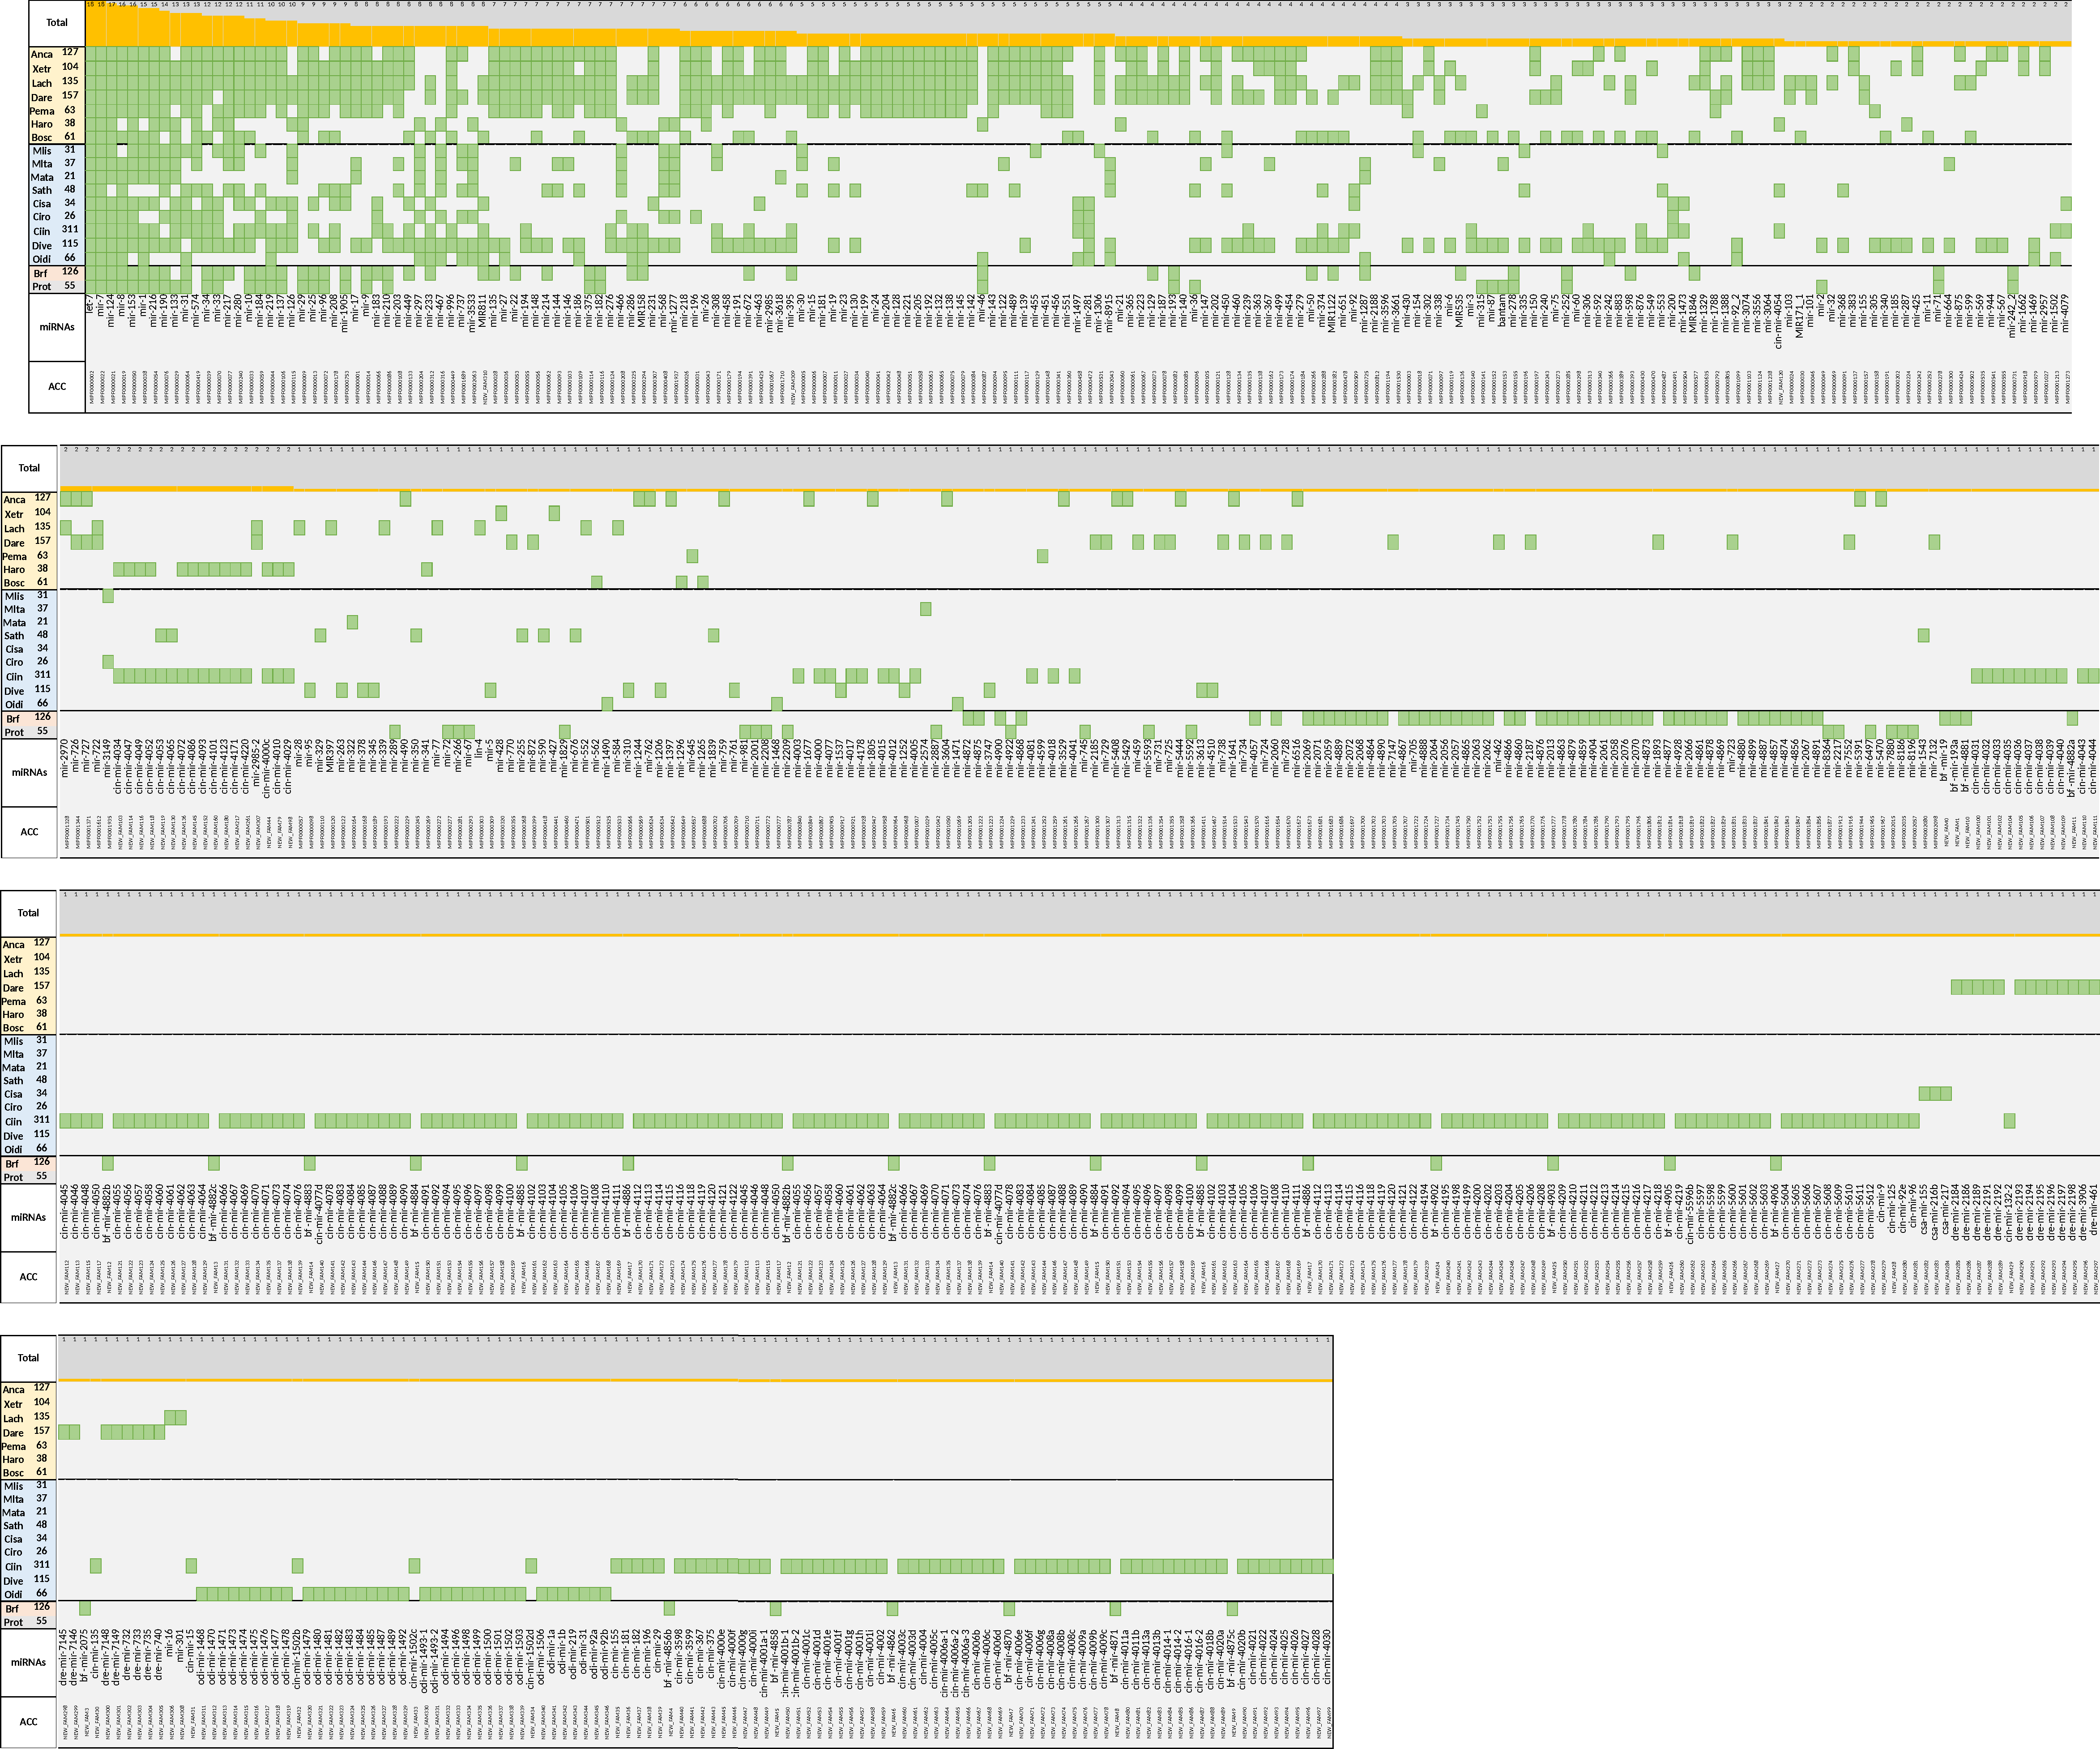
\includegraphics[width=\textwidth, angle=90]{./Images/miRNA_matrix}
\caption{Absence/Presence Matrix of miRNAs families along Bilaterian species. 
\textbf{Prot}: Protostomata, \textbf{Brfl}: \textit{B. floridae}, 
\textbf{Oidi}: \textit{O. dioica}, \textbf{Dvex}: \textit{D. vexillum}, 
\textbf{Ciin}: \textit{C. intestinalis}, \textbf{Cisa}: \textit{C. savignyi}, 
\textbf{Ciro}: \textit{C. robusta}, \textbf{Sath}: \textit{S. thompsoni}, 
\textbf{Mata}: \textit{M. oculata}, \textbf{Mlta}: \textit{M. occulta}, 
\textbf{Mlis}: \textit{M. occidentalis}, \textbf{Bosc}: \textit{B. schlosseri}, 
\textbf{Haro}: \textit{H. roretzi}, \textbf{Pema}: \textit{P. marinus}, 
\textbf{Dare}: \textit{D. rerio}, \textbf{Lach}: \textit{L. chalumnae}, 
\textbf{Xetr}: \textit{X. tropicalis} and \textbf{Anca}: \textit{A. 
carolinensis}. }
\label{fig:matrimirnas}
\end{figure}

Our miRNA families updated with the new two annotated miRNAs Salpa and 
Halocyntia

\begin{figure}[t]
\sidecaption[t]
%\centering
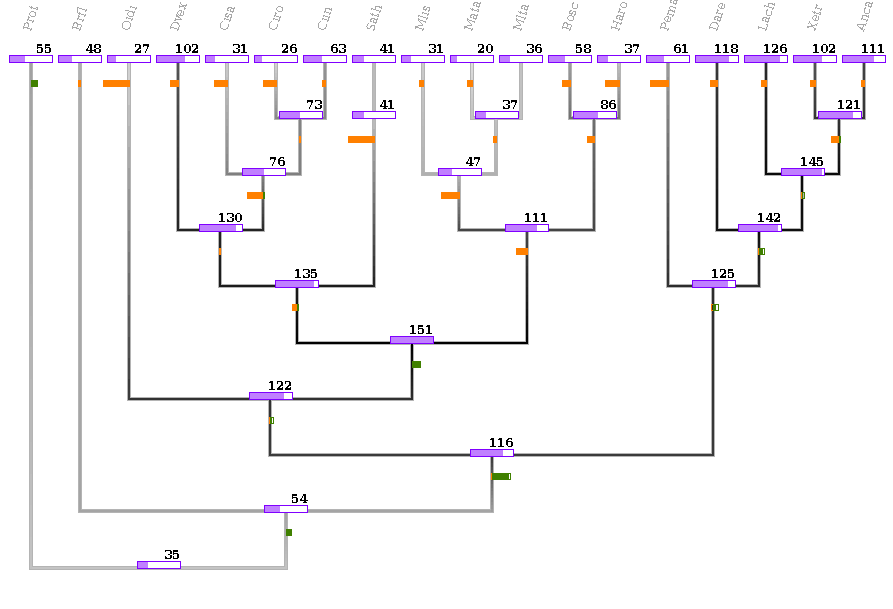
\includegraphics[width=7.5cm]{./Images/last_tree.png}
\caption{Dollo parsymony of miRNAs families distribution in some 
chordates genomes}.
\label{fig:dollotree}
\end{figure}

\begin{figure}[t]
\sidecaption[t]
%\centering
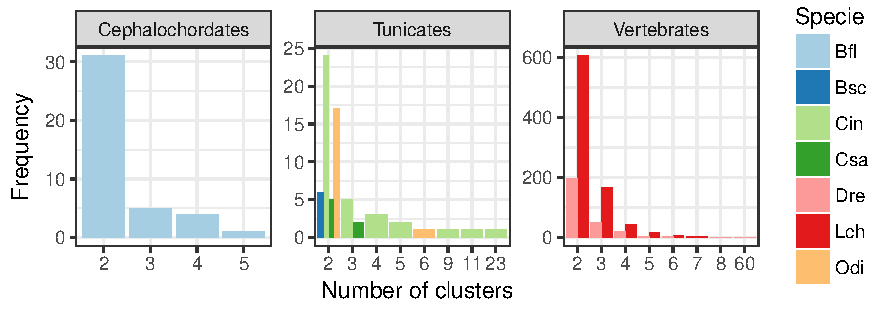
\includegraphics[width=7.4cm]{./Images/cluster_number.pdf} \\ 
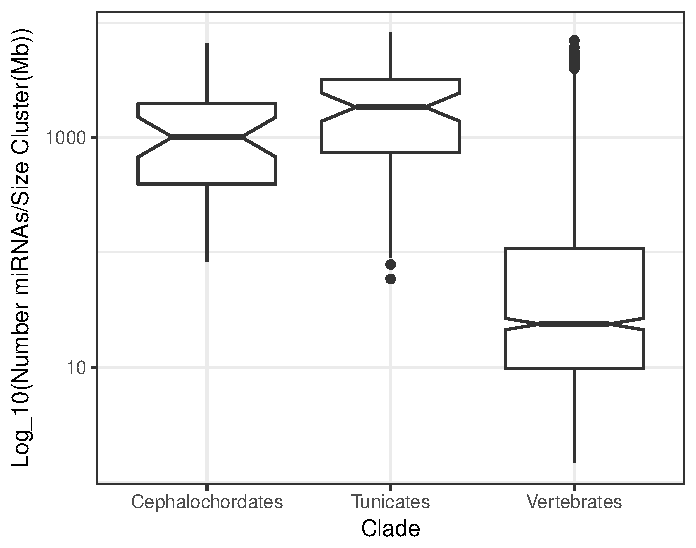
\includegraphics[width=7.4cm]{./Images/density.pdf} 
\caption{Analysis of the distribution, size and number's of cluster along chordate species.}
\label{fig:sizeCluster}
\end{figure}

\begin{figure}[t]
\sidecaption[t]
%\centering
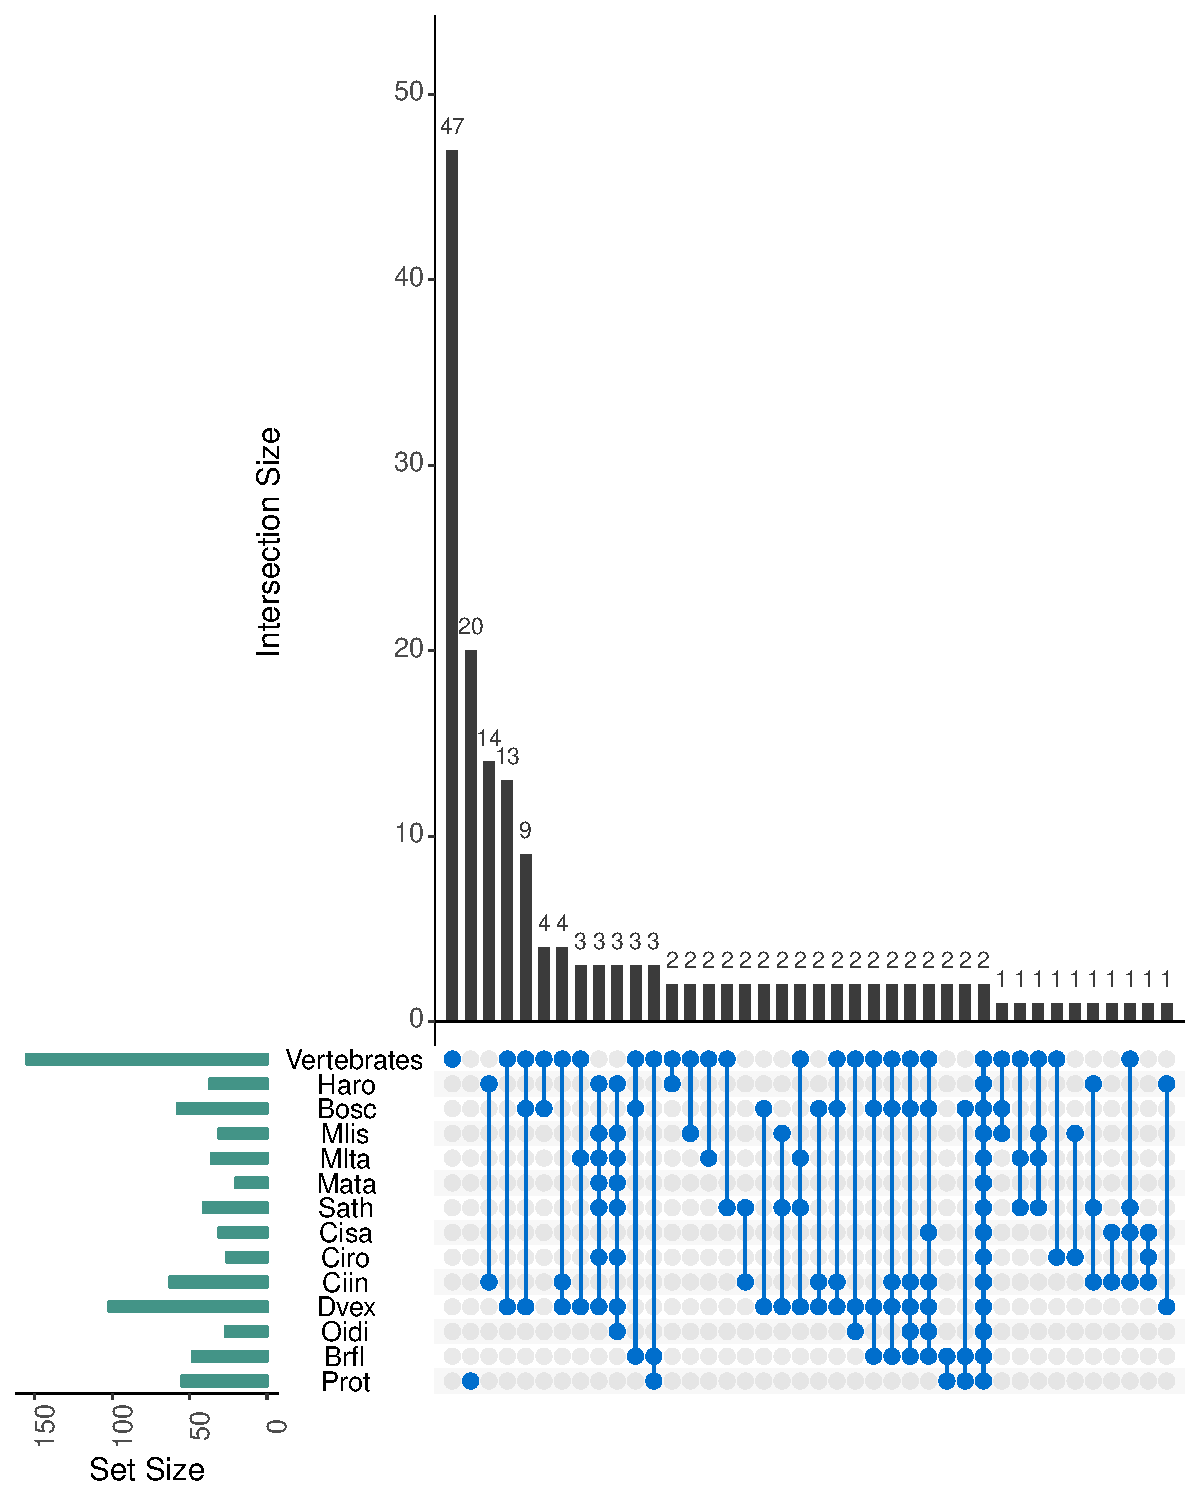
\includegraphics[width=7.5cm]{./Images/vennmiRNAs}
\caption{Comparsion between miRNAs families along Bilaterian species. Same 
labels from Figure \ref{fig:matrimirnas} were used. In this case 
\textsl{vertebrates} group the following species: \textbf{Pema}: \textit{P. 
marinus}, \textbf{Dare}: \textit{D. rerio}, \textbf{Lach}: \textit{L. 
chalumnae}, \textbf{Xetr}: \textit{X. tropicalis} and \textbf{Anca}: \textit{A. 
carolinensis}}
\label{fig:vennDiagram}
\end{figure}

\iffalse
\cite{Velandia-Huerto2016} \textit{A comparative analysis of miRNAs families in 
tunicates is summarized in Fig. 5 c and d. We find several patterns of 
recognizable trends as we analyze the conservation, loss and gain of miRNA 
families in tunicates compared to selected bilaterians. For instance, based in 
our analysis of conserved miRNA families across the bilaterians, we estimate 
that ancestor of the Bilateria likely contained approximately 33 miRNA families. 
In contrast, the ancestor of the Chordata presumably contained members of 37 
miRNA families. In the cephalochordate B. floridae, we find the occurrence of a 
unique repertoire of 82 miRNA families that evolved as a consequence of many 
gains (+50), but also some losses (−5) [8]. In the ancestor of Olfactores we 
presume the presence of 72 miRNA families, of which tunicates did not show 
losses, with the notable exception of O. dioica that has undergone substantial 
losses (−60). Within the ascidians, only B. schlosseri and C. savignyi show 
dramatic losses of miRNA families, −32 and −17 respectively. D. vexillum has 
lost 8 miRNA families. D. vexillum shows 16 families that are absent in other 
tunicates i.e. mir-430, mir-9, mir-130, mir-190, mir-139, mir-460, mir-315, 
mir-305, mir-458, mir-185, mir-233, mir-569, mir-944, mir-567, mir-2985 and 
mir-4068 (Fig. 5d). Comparisons of the miRNAs repertoires between the colonial 
tunicates (D. vexillum and B. schlosseri) on the one hand, and solitary 
tunicates (O. dioica, C. intestinalis and C. savignyi) on the other hand, show 
10 microRNA families, i.e. mir-133, mir-186, mir-6, mir-279, mir-340, mir-11, 
mir-60, mir-592, mir-883 and mir-549 that are specific to colonial tunicates, 
while only 2 families, i.e. mir-31 and mir-1473, are specific to olitary 
tunicates. It is worthwhile exploring how colonial specific miRNAs may have been 
co-opted in ascidians to function in somatic stem cell function, regeneration, 
budding, or other asexual developmental processes, as miRNAs are know to be 
important players in stem cell function, and developmental processes of 
differentiation in vertebrates}

\subsubsection{Jueetal2016.pdf}
\cite{Jue2016}
\textit{A preliminary genome sequence has been assembled for the Southern Ocean salp, Salpa thompsoni (Urochordata, Thaliacea). Despite the ecological importance of this species in Antarctic pelagic food webs and its potential role as an indicator of changing Southern Ocean ecosystems in response to climate change, no genomic resources are available for S. thompsoni or any closely-related urochordate species. Using a multiple-platform, multiple-individual approach, we have produced a 318,767,936 bp genome sequence, covering more than 50{\%} of the estimated 602 MB (±173 MB) genome size for S. thompsoni Using a non-redundant set of predicted proteins, more than 50{\%} (16,823) of sequences showed significant homology to known proteins and {\~{}}38{\%} (12,151) of the total protein predictions were associated with Gene Ontology functional information. We have generated 109,958 SNP variant and 9,782 indel predictions for this species, serving as a resource for future phylogenomic and population genetic studies. Comparing the salp genome to available assemblies for four other urochordates, Botryllus schlosseri, Ciona intestinalis, Ciona savignyi and Oikopleura dioica, we found that S. thompsoni shares the previously-estimated rapid rates of evolution for these species. High mutation rates are thus independent of genome size, suggesting that rates of evolution {\textgreater}1.5 times that observed for vertebrates are a broad taxonomic characteristic of urochordates. Tests for positive selection implemented in PAML revealed a small number of genes with sites undergoing rapid evolution, including genes involved in ribosome biogenesis and metabolic and immune process that may be reflective of both adaptation to polar, planktonic environments as well as the complex life history of the salps. Finally, we performed an initial survey of small RNAs, revealing the presence of known, conserved miRNAs, as well as novel miRNA genes; unique piRNAs; and mature miRNA signatures for varying developmental stages. Collectively, these resources provide a genomic foundation supporting S. thompsoni as a model species for further examination of the exceptional rates and patterns of genomic evolution shown by urochordates. Additionally, genomic data will allow for the development of molecular indicators of key life history events and processes and afford new understandings and predictions of impacts of climate change on this key species of Antarctic pelagic ecosystems.}


\subsubsection{Wangetal2017.pdf}
\cite{Wang2017}
\textit{Background: miRNAs play essential roles in the modulation of cellular functions via degradation and/or translation
attenuation of target mRNAs. They have been surveyed in a single ascidian genus, Ciona. Recently, an annotated
draft genome sequence for a distantly related ascidian, Halocynthia roretzi, has become available, but miRNAs in
H. roretzi have not been previously studied.
Results: We report the prediction of 319 candidate H. roretzi miRNAs, obtained through three complementary
methods. Experimental validation suggests that more than half of these candidate miRNAs are expressed during
embryogenesis. The majority of predicted H. roretzi miRNAs appear specific to ascidians or tunicates, and only 32
candidates, belonging to 25 families, are widely conserved across metazoans.
Conclusion: Our study presents a comprehensive identification of candidate H. roretzi miRNAs. This resource
will facilitate the study of the mechanisms for miRNA-controlled gene regulatory networks during ascidian
development. Further, our analysis suggests that the majority of Halocynthia miRNAs are specific to ascidian
or tunicates, with only a small number of widely conserved miRNAs. This result is consistent with the general
notion that animal miRNAs are less conserved between taxa than plant ones.}

\fi

\section{miRNAs and its rol in development}
\label{sec:3}

\subsection{let-7 was the first miRNA in tunicates proposed to have a regulatory 
role in development}
The first miRNA ever reported in any tunicate was let-7, which was 
first detected in \textit{C. robusta} and \textit{Herdmania curvata} 
\cite{Pasquinelli2000}. A previous study the same year in \textit{C. elegans} 
had shown that small RNA let-7 ($21$ nt) was required for late larval to adult 
developmental transition \cite{Reinhart:2000mz}. Small RNA let-7 was then shown 
to also be differentially expressed during the development of many distantly 
related animal taxa, but was not detected in Porifera, Ctenophora, Cnidaria, 
and Acoelomorpha, suggesting that let-7 was involved in the regulation of late 
temporal transitions during development or in the evolution of complex life 
histories in the Nephrozoa \cite{Pasquinelli2000, Pasquinelli2003}.

\subsection{miRNAs discovery and development}

Both MicroRNAs (miRNAs or miRs) as well as MicroRNA offset RNA (moRNAs or moRs) 
are developmentally regulated as shown during \textit{C. robusta} development 
\cite{Shi2009}. In spite of the considerably higher abundance of miRs and 
miRs* in cells than their corresponding abundance of moRs, all three small RNA 
types have been shown to have regulatory roles for gene expression. Although a 
vast majority of miRNAs remain to be studied, there are already many cases of 
well-studied miRNAs (including many that are mentioned in this chapter that have 
been studied in tunicates) that are known to target mRNAs, modulate their levels 
of expression, and affect developmental processes both in plants and animals 
\cite{Zhao2018}. Only recently two studies demonstrated for 
the first time that two moRs (viral moR-rR1-3-5p and moR-21) could also 
modulate gene expression, and were not merely the byproduct of miRNA biogenesis 
\cite{UMBACH2010592, Zhao2016}.

\subsection{Neuronal fate determination and regulation by miR-124}

The miRNA miR-124 is expressed in the nervous system of many animals, including 
Drosophila \cite{Aboobaker18017}, \textit{C. elegans} \cite{Clark:2010} and 
humans \cite{Sempere2004}. As was first observed by in vitro studies of mouse 
brain cells, low expression of miR-124 was related to neural stem cell 
maintenance, whereas high expression of miR-124 induced the differentiation of 
neuronal cell types \textcolor{red}{(Cheng et al., 2009)}. A regulative role of 
miR-124 in non-neural vs. neural fate decisions was further investigated by 
embryonic experiments in vivo \cite{Chen4943} and by 
theoretical and in silico modeling analyses in \textit{C. robusta} 
\cite{Chen2014}. These studies showed that miR-124 promotes 
nervous system development by feedback interactions with Notch signaling. During 
nervous system development of \textit{C. robusta}, cells in the dorsal and 
ventral midline epidermis of the teilbud embryo either take an epidermal sensory 
neuron (ESN) or peripheral nervous system (PNS) fate, a decision mediated by 
lateral inhibition using a classical model of feedback loop regulation of 
Notch-Delta signaling in neighboring cells \cite{Collier:1996, 
Chen2014}. Cells that take an ESN fate showed low expression of miR-124 
presumably by Notch inhibition, whereas cells that take a PNS fate expressed 
high levels of miR-124, which in the latter case it was shown to target and 
repress non-neuronal genes (e.g. neuronal repressors SCP1 and PTBP1) downstream 
of Notch signaling \cite{Chen4943}. In addition, expression 
of miR-124 in larval epidermal cells was sufficient for ectopic neural 
specification, which resembled mis-expression experiments using Pou4, an 
important transcription factor for sensory neuron specification 
\cite{Chen4943, JoyceTang2013}. Whereas miR-124 targeting to SCP1 is thought to 
have evolved in the vertebrates+tunicates, miR targeting to PTBP1 may be 
conserved among bilaterians except for ecdysozoans \cite{Chen4943} suggesting 
that the miRNA regulatory logic in lateral inhibition models of Notch-Delta 
signaling may have broader implications in other organisms yet to be studied 
\cite{Chen2014}. The research team also showed that miR-124 
acted at the gastrula stage and targeted other non-neural genes such as muscle 
determinant Macho-1 and notochord determinant Brachyury to allow for ectodermal 
fate specification \cite{Chen4943}.

\subsubsection{Muscle development and the polycistronic miR-1/miR-133 cluster}
A well-studied case of miRNA regulation in muscle development is the 
miR-1/miR-133 polycistronic cluster. Whereas miR-1 promotes differentiation of 
muscle, miR-133 promotes proliferation of muscle precursors \cite{Chen:2005yq}. 
In the chordates, these two miRNAs are encoded in an antisense direction in a 
relatively close localization (3-11 kb apart) within the gene \textit{mind bomb 
1} (MIB1), and transcribed as a single primary (i.e. polycistronic) transcript. 
Except for Drosophila and ambulacrarians (i.e. echinoderms and hemichordates), a 
close proximity of these two miRNAs has been documented in most animal taxa 
suggesting some form of functional regulatory constraint of a condensed 
miR-1/miR-133 cluster for the bilaterians \cite{Campo-Paysaa:2011}. 
During \textit{C. robusta} development, the polycistronic transcription can be 
detected in the nuclei of presumptive tail muscle cells from the gastrula stage 
onward, and its transcription is regulated by an $850$ bp sequence upstream of 
the transcipt start site \cite{Kusakabe2013}. Differential 
expression of the two miRNAs in muscle tissues was only detected in the adult, 
where body wall muscle expressed similar levels of miR-1 and miR-133 and heart 
muscle expressed significantly higher levels of miR-1 \cite{Kusakabe2013}.

\subsubsection{miRNA expression during oral siphon (OS) regeneration}
Three stages of regeneration have been proposed that reconstruct main events of 
regeneration that match expected expression profiles in the corresponding 
timeframes \cite{Knapp:2013}. The three phases correspond to: i. wound Healing, 
ii. transition, and iii. re-development. Using miRNA-mRNA transcriptional 
profiling using a correlation network, differential expression of mRNAs was 
correlated to miRNA profiles during the three regeneration windows mentioned 
above in \textit{C. robusta} oral siphon regeneration \cite{Spina:2017}. In 
the first phase, i.e. wound healing, miRNA target clusters of miR 4178b-5p and 
miR 4\_20211 were found to be correlated to the differential expression of genes 
involved in the following GO term functional classifications: immune response, 
stress response and apoptosis. In the second phase, i.e. transition, miR 
4008c-5p, miR 4123-5p, miR 4178-5p, miR 2\_15911, miR 4\_20211, and miR 11\_7539 
were correlated and known to target Wnt, TGFb and MAPK pathway genes that may be 
regulating the proliferative state characteristic of this particular timeframe. 
In the third phase, i.e. re-development, miR4008c-5p, miR 10\_4533, and miR 
11\_6940 known to target ECM peptidase inhibitors are correlated with the 
characteristic extracellular matrix remodeling that occurs at the final phase of 
regeneration and which resembles the original developmental processes. In 
contrast other miRs were found expressed throughout the regenerative process. 
MiRNA miR 10\_4533 known to target IGF and IGFb was found expressed presumably 
regulating the proliferation of progenitors. Also miR-9 was found expressed 
throughout regeneration and is known to be essential for neural development and 
function, presumably by targeting and regulating genes involved in cytoskeleton 
and cell cycle functions \cite{Galderisi:2003rt, MCBEATH2004483}, instead of 
targeting Notch or Hes-1 \cite{Spina:2017}.

\subsubsection{miRNA expression during \textit{O. dioica} development}
A most thorough study of the miRNA repertoire expressed during development has 
been published for the larvacean \textit{O. dioca} \cite{Fu2008}. Using a 
miRNA array approach with $55$ candidate miRNAs and $10$ developmental stages 
for analyses, some general patterns of miRNA occurrence emerged. MicroRNAs were 
expressed throughout the life cycle of the animal, and were deposited in eggs as 
maternal determinants for early zygotes. Expression of zygotic miRNAs, such as 
miR-1487 and miR-1488, was observed starting on the blastula stage (1.5h post 
fertilization). Most miRNAs analyzed showed developmental regulation (for 
specific miRNAs that were differentially expressed at each stage see 
\cite{Fu2008}), except for some such as miR-1497 that was expressed throughout 
all stages \cite{Fu2008}. From this study, the first sex specific miRNAs were 
revealed: miR-1478 was expressed day $6$ females in the oocytes, whereas 
miR-1487/88 were expressed in day $6$ males. Interestingly, the compact genomes 
of \textit{O. dioica} showed one single copy of most miRNA loci, except for 
miR-1490a, miR-1493, miR-1497d, and miR-1504 that were in two copies 
\cite{Fu2008}.


\section{Other ncRNAs associated to development}
\label{sec:4}

\subsection{Yellow Crescent RNA}

Yellow crescent RNA, i.e. YC RNA, concerns an about 1.2 kb long polyadenylated 
RNA, which can be present throughout the embryonic development of ascidians 
\cite{Swalla1995}. Its name refers to the fact that in situ hybridization 
confirmed that YC RNA is localized in the yellow crescent region of one-cell 
zygotes. The YC transcripts are actually already found in the cortex of 
unfertilized eggs, segregating with the myoplasm to the yellow crescent after 
fertilization \cite{Swalla1995}. Subsequently most YC transcripts enter the 
primary muscle cell lineage after cleavage and are also present in the 
secondary muscle cell lineage \cite{Swalla1995}. YC RNA was first 
discovered in the club tunicate Styela clava \cite{Swalla1995}. As the presence 
of the 1.2-kb RNA in oocytes and early cleaving embryos indicates that it is a 
maternal transcript, YC RNA is considered to be a maternal RNA 
\cite{Swalla1995}. It is associated with the cytoskeleton and segregates to 
the muscle cells during ascidian embryogenesis. Although the YC ORF encodes for 
a putative polypeptide of $49$ amino acids, this protein is relatively small 
and does not show any significant homology to any known proteins. As the YC RNA 
shows various features indicating that it actually functions as an RNA rather 
than as a protein coding molecule, it is considered to be a noncoding RNA that 
may play an important role in growth and development \cite{Swalla1995}.

\subsection{MicroRNA-offset RNAs}

MicroRNA-offset RNAs, i.e. moRNAs, concern about $20$ nucleotides long RNAs 
that lie adjacent to pre-miRNAs. They can originate from both ends of these 
pre-miRNAs, although prevalently they are derived from the 5' arm 
\cite{bortoluzzi2011}. During a study focused on identifying miRNAs in the 
simple chordate \textit{C. intestinalis} moRNAs were first discovered 
\cite{Shi2009}. Unexpectedly, half of the \textit{C. intestinalis} miRNA loci 
that were detected in this study turned out to encode for 
previously uncharacterized small RNAs, in addition to conventional miRNA and 
miRNA* products. This new class of RNAs was hereafter referred to as `moRNAs', 
for miRNA-offset RNAs. It became clear that these moRNAs are probably produced 
by RNAse II-like processing and are observed, like miRNAs, at specific 
developmental stages \cite{Shi2009}.
These results and subsequent studies gave rise to the hypothesis that moRNAs 
concern  a new class of functional regulators whose qualitative alteration 
and/or expression dysregulation might even impact human diseases 
\cite{bortoluzzi2011}. Evidence supporting this hypothesis is still fragmentary 
however. After the discovery in \textit{Ciona}, moRNAs were 
also found in human cells by deep sequencing analysis. Hereby it was reported 
that moRNAs from $78$ genomic loci were weakly expressed in the prefrontal 
cortex \cite{Langenberger2009}. Additional indications that moRNA have a 
distinct function include the fact that some moRNAs are as conserved as miRNAs 
and are in fact conserved across species to an extent that correlated with 
expression level \cite{Shi2009}. The expression level of certain moRNAs can 
even be greater than for their corresponding miRNA \cite{Umbach2010}. Finally, 
it can be argued \cite{bortoluzzi2011} that it is likely that moRNAs might 
represent a functional class of miRNA-related agents as moRNAs are prevalently 
produced by the 5' arm of the precursor, independent of which arm produces the 
most expressed mature miRNA \cite{Langenberger2009, Umbach2010}. 
What functions moRNAs may have, varies. For example, moRNA expression was 
recorded in solid tumours, together with other small RNAs \cite{Meiri2010}. 
In addition the fact that an 18-fold enrichment of moRNAs was observed in the nucleus 
\cite{Taft2010} indicates that at least some moRNAs may have functions related 
to nuclear processes \cite{bortoluzzi2011}. Although these studies do provide 
good indications, the potential functional roles that moRNAs can play, remain 
still largely unknown. 

\subsection{Long Noncoding RNA RMST}

Long noncoding RNAs, i.e. lncRNAs, are abundantly found within mammalian 
transcriptomes. One of the known groups of lncRNAs, includes the 
rhabdomyosarcoma 2-associated transcript (RMST), which is indispensable for 
neurogenesis \cite{Bogu2013}. 
Human RMST was shown as being responsible for the modulation of neurogenesis as 
its expression is regulated by the transcriptional repressor REST while it 
increases during neuronal differentiation \cite{Bogu2013}. Hereby it was 
found that RMST is actually necessary for the binding of SOX2 to promoter 
regions of neurogenic transcription factors. SOX2, a transcription factor known 
to regulate neural fate, in combination with RMST were actually found to 
coregulate a large pool of downstream genes implicated in neurogenesis, i.e. 
more than $1\,000$ genes were differentially expressed upon RMST knockdown 
\cite{Bogu2013}. These results illustrated the role of RMST as a 
transcriptional coregulator of SOX2 and a key player in the regulation of 
neural stem cell fate \cite{Bogu2013}. A further confirmation of the importance 
of RMST came with the discovery of a homologue of this lncRNA in the simple 
chordate \textit{D. vexillum}, i.e. the carpet sea-squirt 
\cite{Velandia-Huerto2016}. While homologues of ``human'' lncRNAs are 
rarely found across all chordates due to their low levels of sequence 
conservation, a plausible homolog of RMST $9$, the conserved region $9$ of the 
Rhabdomyosarcoma 2 associated transcript known for its interaction with SOX2, 
was found in \textit{D. vexillum}. Subsequently putative homologs were also 
found in the genomes of the ascidians \textit{C. intestinalis}, \textit{C. 
savignyi} and \textit{B. schlosseri} and the Florida lancelet \textit{B. 
floridae}, illustrating that RMST lncRNA are thus conserved across chordates, 
making them one of the best conserved lncRNAs known to date 
\cite{Velandia-Huerto2016}.

\subsection{Splices-leader RNA}

mRNA 5'leader trans-splicing is a mode of gene expression in which the 5' end 
of a pre-mRNA is discarded and replaced by the 5' segment of a spliced leader 
(SL) RNA \cite{Vandenberghe2001}. Spliced-Leader RNAs, i.e. SL RNAs, hereby 
consist of a 5' exon and a 3' intron with a conserved consensus 5' splice donor 
site at the exon-intron boundary \cite{Ganot2004}. SL RNA trans splicing has 
not only been described for euglenoids, kinetoplastids, cnidarians, nematodes, 
and Platyhelminthes \cite{Ganot2004}, but also for deuterostomes like the simple 
chordate \textit{C. intestinalis} \cite{Vandenberghe2001} and the 
appendicularian \textit{O. dioica} \cite{Ganot2004}. Hereby \textit{O. dioica} 
was shown to not only trans-splice SL RNAs to mRNAs, as does \textit{C. 
intestinalis}, but also to use trans splicing in resolving polycistronic 
transcripts \cite{Ganot2004}. During trans splicing, the capped SL RNA exon 
moiety is covalently linked to the 5' ends of mRNAs, forming a leader sequence 
ranging from $16$ nt in \textit{C. intestinalis} to $41$ nt in trypanosomatids 
\cite{Ganot2004}. The role of SL trans-splicing is still unknown in many cases. 
SL trans-splicing may potentially having functions varying from the mediation 
of mRNA stability or translatability \cite{Maroney1995} and the resolution 
of polycistronic pre-mRNAs \cite{Agabian1990, Blumenthal1995}, to the 
production of functional mRNAs from RNA polymerase I 
transcripts \cite{ShuLee1997}.

\section{Acknowledgments}
This work and the computational analysis were partially supported by the 
equipment donation from the German Academic Exchange Service-DAAD to the Faculty 
of Science at the Universidad Nacional de Colombia and the computational 
laboratory from Bioinformatics Group at Department of Computer Science and 
Interdisciplinary Center for Bioinformatic at the Leipzig University. The 
comparative analysis was partially supported by Colciencias (project no.\ 
110165843196, contract 571-2014). CAVH acknowledges the support by DAAD 
scholarship: Forschungsstipendien-Promotionen in Deutschland, 2017/18 (Bewerbung 
57299294). CIBS acknowledges Universidad Nacional de Colombia for the time 
granted to write this chapter.

% BibTeX users please use
\bibliographystyle{plain}
\bibliography{tuni_updated}
%\bibliography{tuni, tuni_2, Arjan/biblio_arjan}
%%%%%%

\end{document}
